%%
%% This is file `sample-sigconf.tex',
%% generated with the docstrip utility.
%%
%% The original source files were:
%%
%% samples.dtx  (with options: `all,proceedings,bibtex,sigconf')
%% 
%% IMPORTANT NOTICE:
%% 
%% For the copyright see the source file.
%% 
%% Any modified versions of this file must be renamed
%% with new filenames distinct from sample-sigconf.tex.
%% 
%% For distribution of the original source see the terms
%% for copying and modification in the file samples.dtx.
%% 
%% This generated file may be distributed as long as the
%% original source files, as listed above, are part of the
%% same distribution. (The sources need not necessarily be
%% in the same archive or directory.)
%%
%%
%% Commands for TeXCount
%TC:macro \cite [option:text,text]
%TC:macro \citep [option:text,text]
%TC:macro \citet [option:text,text]
%TC:envir table 0 1
%TC:envir table* 0 1
%TC:envir tabular [ignore] word
%TC:envir displaymath 0 word
%TC:envir math 0 word
%TC:envir comment 0 0
%%
%% The first command in your LaTeX source must be the \documentclass
%% command.
%%
%% For submission and review of your manuscript please change the
%% command to \documentclass[manuscript, screen, review]{acmart}.
%%
%% When submitting camera ready or to TAPS, please change the command
%% to \documentclass[sigconf]{acmart} or whichever template is required
%% for your publication.
%%
%%
\documentclass[acmsmall]{acmart}
%%
%% \BibTeX command to typeset BibTeX logo in the docs
\AtBeginDocument{%
  \providecommand\BibTeX{{%
    Bib\TeX}}}

%% Rights management information.  Replace DOI, volume, number,
%% and article with the exact values from the publisher's rights form.
\setcopyright{cc}
\setcctype{by}
\acmJournal{PACMSE}
\acmYear{2026} \acmVolume{3} \acmNumber{FSE} \acmArticle{FSE091}
\acmMonth{7} \acmDOI{10.1145/3808098}

\usepackage{makecell}
\usepackage{booktabs}
\usepackage{tabularx}
\usepackage{array}
\usepackage{enumitem}
\usepackage{multirow}
\usepackage{threeparttable}
\usepackage{booktabs}
%%
%% Submission ID.
%% Use this when submitting an article to a sponsored event. You'll
%% receive a unique submission ID from the organizers
%% of the event, and this ID should be used as the parameter to this command.
%%\acmSubmissionID{123-A56-BU3}

%%
%% For managing citations, it is recommended to use bibliography
%% files in BibTeX format.
%%
%% You can then either use BibTeX with the ACM-Reference-Format style,
%% or BibLaTeX with the acmnumeric or acmauthoryear sytles, that include
%% support for advanced citation of software artefact from the
%% biblatex-software package, also separately available on CTAN.
%%
%% Look at the sample-*-biblatex.tex files for templates showcasing
%% the biblatex styles.
%%

%%
%% The majority of ACM publications use numbered citations and
%% references.  The command \citestyle{authoryear} switches to the
%% "author year" style.
%%
%% If you are preparing content for an event
%% sponsored by ACM SIGGRAPH, you must use the "author year" style of
%% citations and references.
%% Uncommenting
%% the next command will enable that style.
%%\citestyle{acmauthoryear}


%%
%% end of the preamble, start of the body of the document source.
\begin{document}

%%
%% The "title" command has an optional parameter,
%% allowing the author to define a "short title" to be used in page headers.
\title{Multi-LLM Persona Generation for Virtual Focus Groups in Software Engineering: A Controlled, Multi-domain Study of Emotional Requirements Elicitation}

%%
%% The "author" command and its associated commands are used to define
%% the authors and their affiliations.
%% Of note is the shared affiliation of the first two authors, and the
%% "authornote" and "authornotemark" commands
%% used to denote shared contribution to the research.
\author{Guangrui Fan}
\authornote{Corresponding author.}
\email{fgr@tyust.edu.cn}
\orcid{0000-0000-0000-0000}       %% TODO: replace with real ORCID
\affiliation{%
  \institution{Taiyuan University of Science and Technology}
  \city{Taiyuan}
  \country{China}
}

\author{Dandan Liu}
\email{s2134717@siswa.um.edu.my}
\orcid{0000-0000-0000-0000}       %% TODO: replace with real ORCID
\affiliation{%
  \institution{Universiti Malaya}
  \city{Kuala Lumpur}
  \country{Malaysia}
}

\author{Lihu Pan}
\email{panlh@tyust.edu.cn}
\orcid{0000-0000-0000-0000}       %% TODO: replace with real ORCID
\affiliation{%
  \institution{Taiyuan University of Science and Technology}
  \city{Taiyuan}
  \country{China}
}

\author{Rui Zhang}
\email{zhangrui@tyust.edu.cn}
\orcid{0000-0000-0000-0000}       %% TODO: replace with real ORCID
\affiliation{%
  \institution{Taiyuan University of Science and Technology}
  \city{Taiyuan}
  \country{China}
}

\author{Qian Guo}
\email{2022055@tyust.edu.cn}
\orcid{0000-0000-0000-0000}       %% TODO: replace with real ORCID
\affiliation{%
  \institution{Taiyuan University of Science and Technology}
  \city{Taiyuan}
  \country{China}
}

%%
%% By default, the full list of authors will be used in the page
%% headers. Often, this list is too long, and will overlap
%% other information printed in the page headers. This command allows
%% the author to define a more concise list
%% of authors' names for this purpose.
\renewcommand{\shortauthors}{Fan et al.}

%%
%% The abstract is a short summary of the work to be presented in the
%% article.

%% Abstract
\begin{abstract}
Emotional requirements (ERs)---how users should feel and which emotional harms a system must avoid---often determine whether people adopt and keep using software, especially in sensitive domains. Yet, eliciting ERs via interviews, workshops, and focus groups is costly and hard to scale or repeat. We study whether simulated focus groups, moderated discussions among user personas generated and played by large language models (LLMs), can augment early ER elicitation. Across three domains (mental‑health journaling, personal finance, and fitness), we compare one‑shot and iterative single‑model pipelines with iterative pipelines that use two or three different LLMs, and we benchmark against two human baselines: a human focus group and Emotional Goal Modeling (EGM). Multi‑LLM pipelines generate more diverse personas and increase the share of AI‑only ERs (not seen in our human baselines) that source‑blinded raters judge relevant by \(14.7\) percentage points compared to an iterative single‑model workflow; same‑model controls suggest this gain is not solely due to provider differences. Compared to human methods, simulations contribute more innovative requirements, EGM contributes clearer and more feasible ones, and human focus groups provide more natural phrasing. Overall, the results support an augmentation‑oriented workflow: use multi‑LLM simulation to broaden candidate ERs, structured modeling to organize them, and human engagement to ground decisions.
\end{abstract}
%% Keywords (kept concise; aligned with contributions)


%%
%% The code below is generated by the tool at http://dl.acm.org/ccs.cfm.
%% Please copy and paste the code instead of the example below.
%%
\begin{CCSXML}
<ccs2012>
   <concept>
       <concept_id>10011007.10011074.10011075.10011076</concept_id>
       <concept_desc>Software and its engineering~Requirements analysis</concept_desc>
       <concept_significance>500</concept_significance>
       </concept>
   <concept>
       <concept_id>10003120.10003130.10003134</concept_id>
       <concept_desc>Human-centered computing~Collaborative and social computing design and evaluation methods</concept_desc>
       <concept_significance>500</concept_significance>
       </concept>
 </ccs2012>
\end{CCSXML}

\ccsdesc[500]{Software and its engineering~Requirements analysis}
\ccsdesc[500]{Human-centered computing~Collaborative and social computing design and evaluation methods}


%%
%% Keywords. The author(s) should pick words that accurately describe
%% the work being presented. Separate the keywords with commas.
\keywords{Requirements Engineering, Emotional Requirements, Large Language Models, Multi-Model Orchestration, Virtual Focus Groups, Emotional Goal Modeling}
%% A "teaser" image appears between the author and affiliation
%% information and the body of the document, and typically spans the
%% page.


%%
%% This command processes the author and affiliation and title
%% information and builds the first part of the formatted document.
\maketitle
\section{Introduction}

Many software systems fail not because they lack features, but because they make users feel judged, unsafe, or disrespected, especially in sensitive contexts \cite{curumsing2014designing}. Emotional requirements (ERs) capture requirements and concerns tied to users’ emotional state, emotional triggers, emotional safety, or emotion‑shaping design choices (e.g., avoiding shame after missed streaks; feeling safe when sharing reflections). ERs are increasingly recognized as first‑class concerns in software engineering \cite{miller2015emotion,alkhomsan2024eliciting}, yet they remain difficult to elicit well: conventional requirements engineering (RE) methods---interviews, focus groups, and workshops---are costly to organize, hard to repeat, and difficult to run at scale \cite{curumsing2014designing,hadiana2020emotional}. In domains such as mental‑health journaling, missing or mis‑specified ERs can undermine perceived safety and ultimately product success \cite{madampe2022emotional}.

This paper asks whether simulated focus groups---moderated discussions among personas generated and played by large language models (LLMs)---can broaden early ER elicitation. In a controlled, multi‑domain study, multi‑LLM pipelines produce more diverse personas and increase the share of AI‑only ERs (absent from the human baselines) that source‑blinded raters judge relevant by \(14.7\) percentage points compared to an iterative single‑model workflow. The practical implication is a hybrid diverge–structure–ground (DSG) workflow: diverge with multi‑model simulation (breadth/innovation), structure with Emotional Goal Modeling (EGM) (clarity/feasibility and traceability), and ground decisions through human engagement. We do not claim that simulated focus groups replace affected users or human focus groups in sensitive domains. Instead, we position them as a fast, reproducible way to expand the space of candidate ERs early, which then must be vetted, contextualized, and prioritized with people.

Large language models (LLMs) offer a low‑marginal‑cost way to draft candidate personas and explore alternative viewpoints. Early work shows that LLMs can assist qualitative analysis and elicit user needs from text \cite{bano2024large,hayes2025conversing,crocker2025proof,omizo2024automating}. However, many LLM‑based elicitation approaches either mine existing artifacts or rely on a single model role‑playing a proxy stakeholder \cite{bano2023ai,marques2024using,barros2025large}. A single synthetic “voice” can miss tensions central to ERs (e.g., nudges that motivate some users but feel judgmental to others) and can yield overly homogeneous outputs \cite{kung2023performance,lin2025leveraging}. This motivates studying whether using multiple models and interaction can broaden coverage without sacrificing quality.

We evaluate simulated focus groups with a pipeline that generates persona cards, runs scripted discussions, clusters and deduplicates candidate requirements, and validates outputs with independent raters who are blinded to the source (AI vs.\ human methods). We benchmark against two human baselines: a conventional human focus group and EGM, a structured method that supports explicit goal$\rightarrow$requirement traceability.

We study three consumer domains with distinct emotional profiles: mental‑health journaling as the primary domain with full replications, and personal finance and fitness as satellite domains with lean replications of key contrasts. We compare four AI configurations that disentangle iteration and model plurality: C0 (one‑shot, single model), C1 (iterative, single model), C2 (iterative, two models), and C3 (iterative, three models). We benchmark all AI configurations against both human baselines. In the primary domain, we additionally run compact same‑model controls to help separate multi‑voice workflow structure from provider capability.

This work makes three contributions. First, we present a controlled experimental design that disentangles the effects of iterative workflow from multi‑model plurality in persona generation and simulated focus groups, incorporating multi‑domain replications and same‑model ablation controls in the primary domain. Second, we benchmark simulated focus groups against two established human baselines---conventional focus groups and Emotional Goal Modeling---evaluating all outputs through independent, source‑blinded ratings on relevance, clarity, feasibility, and innovation. Third, we demonstrate that multi‑model configurations increase persona diversity and raise the share of AI‑only requirements passing source‑blinded validation by a pooled \(+14.7\) percentage points over an iterative single‑model workflow, while EGM retains its advantage on clarity and feasibility. 


Building on the gaps identified, we formulate three research questions that progressively move from upstream persona quality, through downstream requirement outcomes, to the interaction mechanisms that link the two.

\smallskip\noindent\textbf{RQ1 (Iteration vs.\ multi‑model).} Do iterative workflows that use multiple LLMs produce more diverse personas than one‑shot or iterative single‑model workflows across domains?

\smallskip\noindent\textbf{RQ2 (Elicitation quality \& baselines).} Do simulated focus groups yield more source-validated, AI‑only emotional requirements under multi‑model configurations, and how do their outputs compare with EGM and human focus groups on quality ratings?

\smallskip\noindent\textbf{RQ3 (Mechanisms).} Which interaction features within simulated dialogs account for differences in validated yield---specifically, the roles of persona diversity, productive disagreement, and empathy events---beyond iteration and domain?

Unlike prior work that treats diversity as a textual attribute of personas \cite{lazik2025good}, our design makes heterogeneity consequential for elicitation by isolating iteration from plurality, preserving model differences as stable dialogic voices, and connecting outputs to source‑blinded human validation and interaction mechanisms (detailed positioning in \S\ref{sec:gaps}). 

In the following paper, section~\ref{sec:method:design} describes the experimental conditions, domains, and baselines, followed by orchestration, extraction, and validation procedures (\S\ref{sec:measures-validation}). Section~4 reports results organized by the research questions. Section~5 discusses implications for practice, including hybrid usage patterns and limitations. Table~\ref{tab:key-terms} defines the key terms used throughout the paper.

\begin{table}[t]
  \centering
  \caption{Key terms and notation (used throughout).}
  \label{tab:key-terms}
  \scriptsize 
  \setlength{\tabcolsep}{5pt}
  \begin{tabularx}{\linewidth}{p{3.4cm}X@{}}
    \toprule
    \textbf{Term} & \textbf{Definition} \\
    \midrule
    Emotional requirement (ER) & A requirement or concern explicitly linked to users’ emotional state, emotional triggers, emotional safety, or designs intended to shape emotions (definitions and examples in the coding manual). \\
    Primary domain / satellite domains & Domain~A (primary) runs the full set of AI conditions with more replications; Domains~B/C (satellites) provide lean replications of key contrasts to probe external validity. \\
    Persona card & A structured textual profile (bio, triggers, boundaries, voice snippet) used to ground a simulated participant in the focus group. \\
    Simulated (AI‑mediated) focus group & A moderated dialogue among persona voices generated/played by LLMs, using a fixed script and logging. \\
    AI conditions (C0--C3) & C0: single‑model, one‑shot personas; C1: single‑model, iterative 3‑step; C2: two‑model sequential across steps; C3: three‑model sequential across steps. \\
    Human baselines (HB1/HB2) & HB1: human focus group; HB2: Emotional Goal Modeling (EGM) session with goal$\rightarrow$requirement tracing. \\
    Run / seed & An independent replicate intended to capture variability; when provider APIs expose pseudo‑random seeds we set/log them, otherwise we log timestamps and version strings as seed proxies. \\
    AI‑only requirement & A deduplicated requirement cluster that appears in AI transcripts but not in HB1/HB2 within the same domain. \\
    Validated requirement & A requirement is validated by source-blinded raters if either (i) its median relevance $\geq 4$ or (ii) $\geq 60\%$ of raters assign relevance $\geq 4$ (see \S\ref{sec:measures-validation}). \\
    Validated AI-only share & \#AI-only requirements that are validated / \#AI-only requirements (yield metric). \\
    \bottomrule
  \end{tabularx}
\end{table}

\section{Related Work}
\label{sec:related}

\subsection{Emotional Requirements in Software Engineering}
Early work argues that emotions are first‑class concerns that shape adoption, engagement, and trust, and calls for methods that surface affective drivers alongside functional and non‑functional needs \cite{miller2015emotion,curumsing2014designing,hadiana2020emotional}. Approaches span explicit “emotion‑led” modeling and instruments such as Affect Grids and Kansei engineering \cite{colomo2011using,hadiana2020emotional}, as well as facilitation frameworks for eliciting tensions and trade‑offs \cite{miller2015emotion,curumsing2014designing}. Empirically, emotions in software usage often emerge through interaction (focus groups, interviews) but are costly to capture at scale and vulnerable to moderator bias and scheduling constraints \cite{alkhomsan2024eliciting,thew2018value,ortu2016emotional}. Emotional Goal Modeling (EGM) provides traceable goal$\rightarrow$subgoal$\rightarrow$requirement structure that can improve feasibility and clarity, yet still requires substantial human effort and domain expertise \cite{curumsing2014designing,hadiana2020emotional}. Recent studies emphasize both the importance and difficulty of obtaining robust emotional data in sensitive domains (e.g., mental health, finance) \cite{madampe2022emotional}.
\subsection{AI/LLMs for Requirements Elicitation: From Artifact Parsing to Elicitation}
LLMs have been used to accelerate qualitative analysis and coding, summarize interview data, and mine requirements from artifacts \cite{barros2025large,schroeder2024large,omizo2024automating,than2025updating,crocker2025proof,castellanos2025large}. Several papers explore role‑play or prompt‑based elicitation where a single model acts as a proxy stakeholder to generate user needs or scenarios \cite{marques2024using,lojo2025using,ferrari2025formal,zhang2024focus}. Surveys caution, however, that single‑model deployments risk homogenized outputs and that human validation remains essential, particularly for emotionally laden contexts \cite{bano2023ai}. Overall, this literature establishes feasibility and efficiency gains but is largely artifact‑centric or single‑voice, leaving open how to orchestrate multiple perspectives interactively and how to evaluate AI‑generated emotional requirements against human baselines under blind review \cite{bano2024large,hayes2025conversing}.
\subsection{LLM Personas and Virtual Focus Groups}
Recent work proposes pipelines for persona creation or simulated focus groups, often using a single LLM with prompt templates to generate “user voices” \cite{wu2025personas,liu2024personaflow,zhang2024focus}. These studies demonstrate face validity (coherent personas, plausible dialogues) and practical utility (faster ideation), but two limitations recur. First, most do not disentangle gains from iterative workflow versus model diversity: improvements could stem from multiple passes by the same model rather than truly heterogeneous viewpoints. Second, evaluation typically emphasizes plausibility or coverage rather than external human validation on quality dimensions (relevance, clarity, feasibility, innovation), and rarely benchmarks against structured human methods such as EGM or conventional focus groups. Questions also remain about the authenticity and ethical governance of synthetic “voices” \cite{hulman2023chatgpt,bano2023ai}. Recent RE work has also started to scrutinize diversity and quality in LLM‑generated personas directly. Lazik et al.~\cite{lazik2025good} examine how diversity is requested and realized in LLM‑generated personas via a qualitative user study with and without explicit diversity incentives, operationalizing persona diversity as the presence of diversity aspects in prompts and persona outputs. They find that users tend to request limited diversity unless explicitly instructed, and they highlight a pitfall of performative diversity: personas may mention diverse attributes without translating them into meaningful implications for requirements work. This motivates (i) methods that make heterogeneity consequential in interaction, rather than cosmetic in descriptions, and (ii) evaluations that connect persona diversity to downstream elicitation outcomes.
\subsection{Multi‑Model Orchestration and Multi‑Agent Dialog}
Ensemble and multi‑agent approaches in NLP show that diversity across models can capture complementary signal and improve robustness \cite{yang2025large,deiner2024large}. Multi‑agent simulations suggest that agent heterogeneity can produce more realistic interactions and emergent behaviors \cite{park2023generative,hulman2023chatgpt}. In requirements contexts, multi‑model settings have been proposed to broaden the space of needs and expose conflicts \cite{gorer2024gpt,khan2025large,marques2024using}. Yet, few studies experimentally isolate the marginal effect of model plurality from iterative workflow, or tie interaction patterns (e.g., disagreement, empathy) to externally judged requirement value. Moreover, prior work seldom reports blinded human ratings, effect sizes with uncertainty, or cross‑domain replications that permit pooled estimates \cite{bano2023ai}. Finally, there is limited guidance on how AI plurality should be combined with structured human methods (e.g., EGM) to balance innovation with feasibility and clarity.
\subsection{Research Gaps and Positioning}
\label{sec:gaps}
Our study addresses the foregoing gaps—and responds to recent evidence that LLM‑generated personas can exhibit superficial or performative diversity in RE settings \cite{lazik2025good}—on four fronts in a single, controlled design. First, we experimentally disentangle gains from iterative workflow versus true model plurality by contrasting a single‑model sequential pipeline (C1) with a three‑model pipeline (C3) and, in the primary domain, inserting a two‑model intermediate (C2) to trace the dose–response of plurality. Our AI conditions are also chosen to map onto baseline patterns common in prior LLM‑persona pipelines (single‑model one‑shot; single‑model iterative refinement; same‑model multi‑voice roleplay; multi‑model orchestration), making comparisons interpretable for readers without re‑implementing every prior system. Second, we submit all outputs to blinded human evaluation on relevance, clarity, feasibility, and innovation under a threshold-based validation rule, reporting inter-rater reliability (ICC/$\alpha$) and effect sizes with confidence intervals to support cumulative synthesis. We benchmark against two strong human baselines—conventional focus groups and Emotional Goal Modeling—to assess trade‑offs (innovation versus feasibility/clarity). Fourth, we move beyond outcome tallies toward mechanism by coding productive, resolution‑oriented conflict and empathy events within AI dialogs and relating these interactional features to validated yield. By shifting from artifact parsing to orchestrated dialog among explicitly heterogeneous models—and tying interaction dynamics to blinded human judgment across domains—this work extends LLM‑for‑RE studies and offers a practical, auditable hybrid pipeline that combines AI plurality (diverge), EGM (structure), and human focus groups (ground) \cite{bano2024large,curumsing2014designing,hayes2025conversing}.

\section{Methods}
\label{sec:method:design}
\subsection{Research Design \& Conditions}
We evaluate the effects of workflow (iterative vs.\ one‑shot) and model plurality (single vs.\ multiple LLMs) on persona quality and emotional‑requirements elicitation using a multi‑domain spanning three consumer contexts: (A) mental‑health journaling (primary), (B) personal finance/budgeting (satellite), and (C) fitness/habit tracking (satellite). Within each domain we compare four AI configurations (C0--C3) against two human baselines (HB1, HB2). The primary domain receives full replications for all AI conditions; satellite domains retain the core contrasts while limiting replications to preserve feasibility. The end‑to‑end flow comprises persona generation $\rightarrow$ (simulated or human) focus‑group interaction $\rightarrow$ requirement extraction/deduplication \& ER/GD coding $\rightarrow$ source‑blinded cross‑ratings $\rightarrow$ post‑validation reflective interviews (Figure~\ref{fig:overview}).

\begin{figure}[!ht]
  \centering
  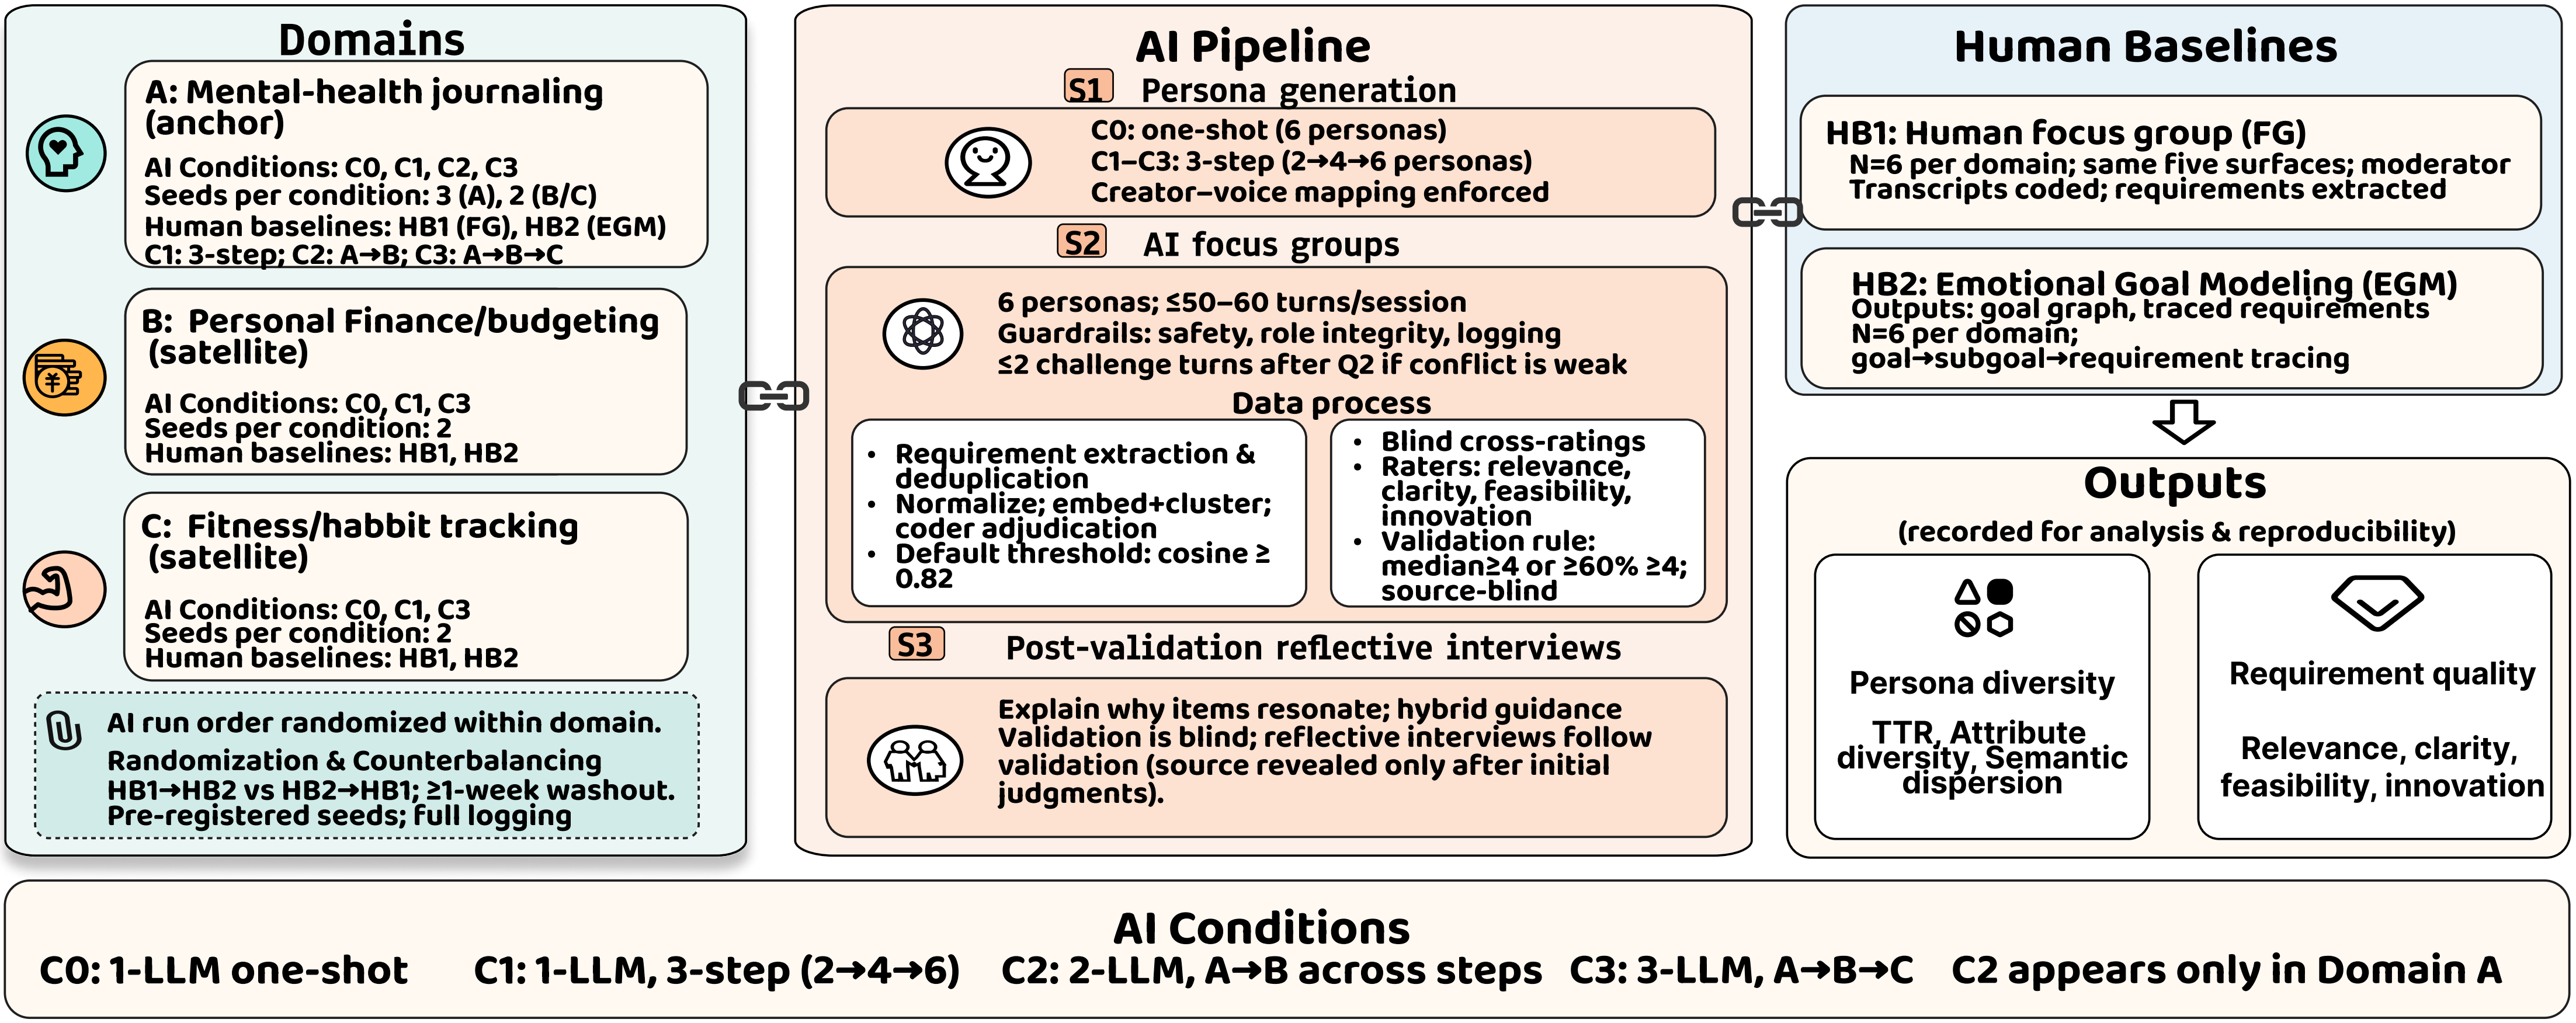
\includegraphics[width=\linewidth]{fig overview.png}
  \caption{Overview of design across domains and conditions. Emotional requirements are surfaced in focus‑group turns, extracted and deduplicated into requirement clusters, coded with ER/GD labels, and validated via source‑blinded ratings.}
  \label{fig:overview}
\end{figure}

AI configurations isolate workflow and plurality: \textbf{C0} (1‑LLM one‑shot); \textbf{C1} (1‑LLM sequential 3‑step, 2$\rightarrow$4$\rightarrow$6 personas); \textbf{C2} (2‑LLM sequential, A$\rightarrow$B across the 3 steps); \textbf{C3} (3‑LLM sequential, A$\rightarrow$B$\rightarrow$C). Human baselines: \textbf{HB1} (human focus group, $N{=}6$/domain) and \textbf{HB2} (Emotional Goal Modeling, same $N{=}6$/domain) (Table ~\ref{tab:design-matrix}).

To separate plurality effects from model/provider strength, we introduce two compact controls in the primary domain (Domain~A): \textbf{C1-MV} (same-model multi-voice), which uses a single base model to create and voice three personas via prompt-diverse role priors and independent seeds within the same 3-step workflow as C1; and \textbf{C3-SM} (same-model C3), which mirrors C3's three-step pipeline but voices all steps with the same base model under distinct role priors. Both controls run with two seeds and identical orchestration limits. 

\begin{table}[ht]
  \centering
  \caption{Design matrix: domains $\times$ AI conditions $\times$ seeds and session counts.}
  \label{tab:design-matrix}
  \small
  \resizebox{\linewidth}{!}{%
  \begin{tabular}{@{}l l c c c@{}}
    \toprule
    \textbf{Domain} & \textbf{AI conditions} & \textbf{Seeds/cond.} & \textbf{\# AI sessions} & \textbf{\# Human sessions} \\
    \midrule
    A.\ Mental‑health journaling (primary) & C0, C1, C2, C3 & 3 & $4 \times 3 = 12$ & HB1 + HB2 $=2$ \\
    B.\ Personal finance/budgeting (satellite) & C0, C1, C3 & 2 & $3 \times 2 = 6$ & HB1 + HB2 $=2$ \\
    C.\ Fitness/habit tracking (satellite) & C0, C1, C3 & 2 & $3 \times 2 = 6$ & HB1 + HB2 $=2$ \\
    \midrule
    \multicolumn{2}{l}{\textbf{Totals}} && \textbf{24} & \textbf{6} \\
    \bottomrule
  \end{tabular}
  }
  \vspace{0.5ex}
{\footnotesize In Domain~A we add two ablation controls—C1-MV (same-model multi-voice) and C3-SM (same-model three-step)—each with two seeds. These runs are not counted in the totals above.}
\end{table}

Primary outcomes capture (i) yield—the validated AI‑only share; and (ii) quality—mean relevance (1--5) of AI‑only requirements.
Secondary: requirement clarity/feasibility/innovation (1--5), persona diversity (lexical/semantic/attribute‑level), group‑dynamics indicators (productive‑conflict density, empathy events, resolution rate). 
Explanatory: themes from post‑validation reflective interviews.

Within each domain, we randomize the AI run order. For human baselines, we split six participants across HB1$\rightarrow$HB2 vs.\ HB2$\rightarrow$HB1 with a $\geq$1‑week washout---a gap between the two sessions to reduce carry‑over and memory effects. Blind raters never see method/source; items are block‑randomized with $\geq$3 raters per requirement. Reflective‑interview stimuli are source‑blind at first and revealed only after initial judgments.

\subsection{Design Rationale and Parameter Choices}
\label{sec:design-rationale}
We chose conditions and parameters to (i) isolate gains from workflow iteration versus model plurality, (ii) keep simulations comparable across conditions and with human baselines, and (iii) make outputs auditable and reproducible. C0 acts as a workflow control (one‑shot, six personas); C1 adds a 3‑step refinement pipeline with the same model; C2/C3 then introduce model plurality. Contrasting C1 vs.\ C0 estimates the gain from iteration; contrasting C2/C3 vs.\ C1 estimates the marginal gain of plurality. The 3‑step progressive expansion (2$\rightarrow$4$\rightarrow$6) mirrors practice, encourages coherence, and fixes the group at six personas to match typical focus‑group sizes. In multi‑model conditions, the creator–voice mapping (each model voices its own personas) keeps heterogeneity actionable and reduces role drift. We selected three LLM families (GPT‑4o, Claude~3.5, Llama‑2) to span complementary interaction styles; provider diversity is not a proxy for cultural diversity, which we treat as a limitation. The deduplication cosine cutoff ($\geq 0.82$) was calibrated manually and varied in $[0.78,0.86]$ as a robustness check (\S\ref{sec:extraction}). Validation uses a threshold rule on relevance (median $\geq 4$ or $\geq 60\%$ of raters $\geq 4$; stricter variants in the supplementary material). Uniform token/turn caps keep sessions comparable in length and cost.

\subsection{Domain Selection}
\label{sec:domains}
We chose domains that (i) exhibit distinct emotional profiles, (ii) are non‑clinical---they do not involve medical advice or clinical interventions, so standard institutional ethics review suffices---and (iii) admit parallelized data collection under identical orchestration. Protocol invariants and adaptation points are centralized in \S\ref{sec:invariants}.

\paragraph{Domain A: Mental‑health journaling (primary).}
A non‑clinical journaling app supporting reflection, mood awareness, and coping. Salient concerns include self‑criticism after lapses, stigma/privacy, and the need for self‑compassionate prompts. This domain receives the full set of AI conditions (C0--C3) with three seeds and both human baselines (HB1, HB2).


\paragraph{Domain B: Personal finance/budgeting (satellite).}
A budgeting app for tracking spending and setting goals. Emotional tensions include money anxiety and guilt, trust in bank aggregation, and the balance between helpful nudges and perceived judgment. AI conditions retain the core contrasts (C0, C1, C3) with two seeds; both HB1 and HB2 are run.


\paragraph{Domain C: Fitness/habit tracking (satellite).}
An app for activity logging and habit formation. Emotions include fluctuating motivation, guilt after missed streaks, social‑comparison pressure, and consent for social visibility. As in Domain~B, we run C0, C1, C3 with two seeds, plus HB1 and HB2. Only a minimal, templated layer changes by domain: a one‑paragraph vignette, example instantiations of the five question surfaces, 2--3 red‑flag terms for bias audit, and 3--5 EGM example cards. 


\subsection{Models, Decoding Parameters, and Seeds}
\label{sec:models-params-seeds}
We employ three complementary LLM families: \textbf{A}=GPT‑4o, \textbf{B}=Claude~3.5, \textbf{C}=Llama‑2 (chat‑tuned). In multi‑model conditions the creator–voice mapping holds: the model that creates a persona also voices that persona during the simulated focus group (Table~\ref{tab:models}). Unless noted, all models use \texttt{temperature}=0.7 and \texttt{top‑p}=1.0 with no frequency or presence penalties. We budget persona generation at $\leq 750$ tokens per step (C1--C3) or per one‑shot pass (C0), and cap focus‑group turns at $\leq 300$ tokens per persona per turn with $\leq 50$--$60$ total turns per session. We use speaker‑delimiter tokens solely to separate turns from different personas.

When a provider API exposes a pseudo‑random seed parameter, we set and log it; otherwise, we keep prompts/parameters fixed and log timestamps and version strings as seed proxies. A run manifest (conditions, seeds/proxies, timestamps, and version strings) is provided in the supplementary material.
\subsection{Persona Generation Protocol (AI)}
\label{sec:persona-protocol}
\begin{table}[!ht]
  \centering
  \caption{Model families and assignment by condition. The creator–voice mapping applies wherever multiple models are used.}
  \label{tab:models}
  \small
  \begin{tabular}{@{}l l l l l@{}}
    \toprule
    \textbf{Label} & \textbf{Family} & \textbf{C0} & \textbf{C1} & \textbf{C2/C3 roles} \\
    \midrule
    A & GPT‑4o & sole model & sole model & C2: Steps 1--2; C3: Step 1 \\
    B & Claude~3.5 & n/a & n/a & C2: Step 3; \; C3: Step 2 \\
    C & Llama‑2 (chat) & n/a & n/a & C3: Step 3 \\
    \addlinespace[2pt]
    SM & Same as A (single base model) & n/a & C1-MV: 3 voices\textsuperscript{$\dagger$} & C3-SM: Steps 1--3 (same model)\textsuperscript{$\dagger$} \\
    \bottomrule
  \end{tabular}

  \vspace{0.25ex}
  {\footnotesize \textsuperscript{$\dagger$}\,C1-MV and C3-SM use prompt-diverse role priors and independent seeds. In heterogeneous C3 runs, step order (A$\rightarrow$B$\rightarrow$C vs.\ B$\rightarrow$C$\rightarrow$A) is randomized by seed in Domain~A.}
\end{table}

\noindent In Domain~A, we randomize the heterogeneous C3 step order by seed (A$\rightarrow$B$\rightarrow$C vs.\ B$\rightarrow$C$\rightarrow$A) to mitigate role-order confounds. As shown in Figure~\ref{fig:persona-pipeline}, conditions C1--C3 follow a standardized 3‑step pipeline that expands a cohort from two to six personas: Step~1 (2 personas), Step~2 (refine +2 $\rightarrow$ 4), Step~3 (refine +2 $\rightarrow$ 6). Condition C0 serves as a workflow control by requesting six personas in a single pass using identical content. The creator–voice rule links generation to subsequent dialogue.

We instantiate prompts from a domain sheet by filling placeholders (e.g., \texttt{[DOMAIN]}, \texttt{[TYPICAL CONTEXTS]}, \texttt{[SENSITIVE ASPECTS]}). The system prompt includes guardrails to minimize stereotype reproduction and stigmatizing language: it prohibits stereotyping or essentializing protected attributes, requires situational grounding for claims, and prefers non‑judgmental phrasing. Full instructions, instantiated prompts, and the retry policy are provided in the supplementary materials.

Each persona is serialized as a persona card with: stable identifier, succinct biography, minimal demographic attributes, salient emotional triggers, motivations, usage patterns/boundaries, and a short first‑person voice snippet to ground speaking style in the focus group. Cards are archived with raw generations, prompts, parameters, and call metadata.

\begin{figure}[!ht]
  \centering
 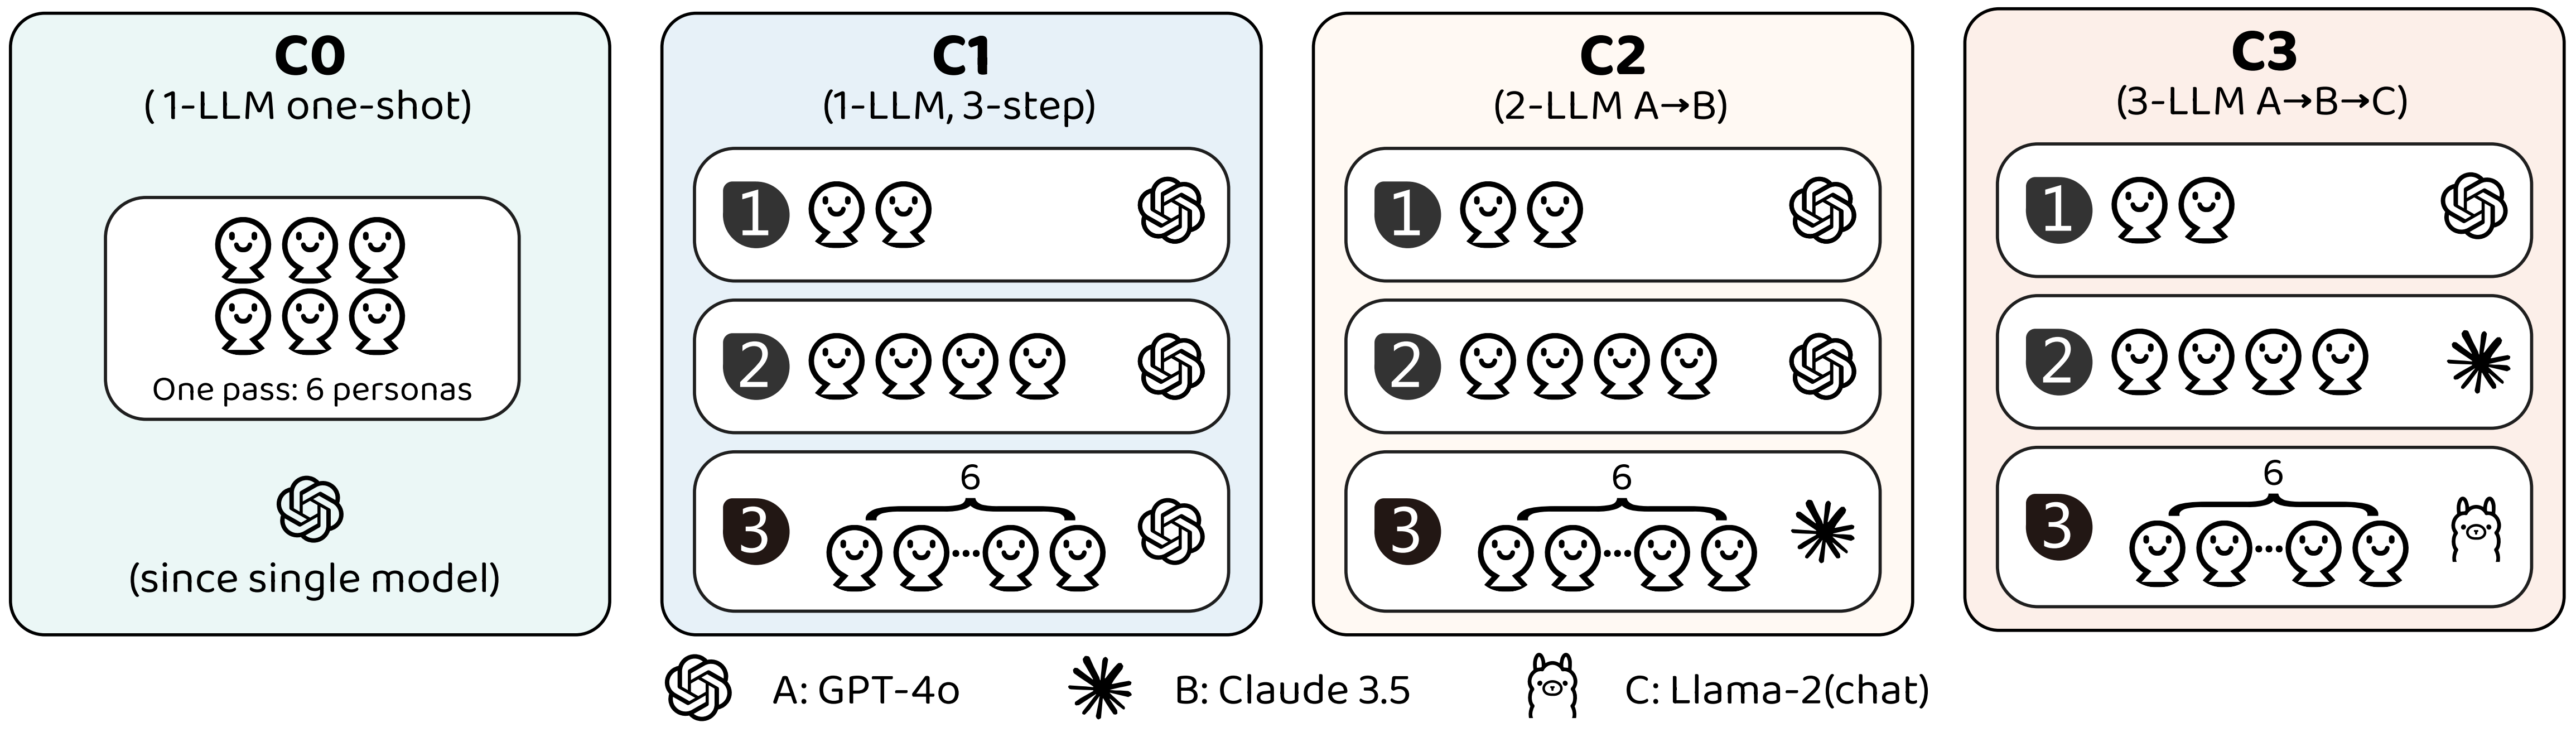
\includegraphics[width=\linewidth]{fig2.png}
  \caption{Persona generation pipeline for C1--C3; C0 is a one‑shot control.}
  \label{fig:persona-pipeline}
\end{figure}

\subsection{AI Focus Group Orchestration}
\label{sec:fg-orchestration}

Each session takes as input (i) six finalized persona cards, (ii) five core question surfaces instantiated for the domain, and (iii) a standardized probe set. The orchestrator feeds the full conversation history as context to every model call; if the transcript approaches 85\% of the provider’s context window, earliest turns are summarized by a fixed, model‑agnostic prompt and the session proceeds with the summary plus recent verbatim turns. Personas speak in round‑robin order for each question. Turns are capped at $\leq 300$ tokens/persona; sessions end after $\leq 50$--$60$ total turns (including moderator turns).

To avoid contrived debates, the moderator injects at most two challenge turns (after Question~2) when spontaneous conflict is weak; these turns only restate or juxtapose existing positions. A lightweight role‑break detector checks speaker tags after every turn; if a persona's tag is missing or mismatched, the orchestrator regenerates that turn once under identical parameters. Similarly, if a provider refuses a prompt for safety reasons, the orchestrator retries once with identical parameters; if the provider continues to refuse after the retry, the refusal is recorded and the session proceeds without that turn. All attempts, flags, and latencies are logged. We archive each session as a verbatim transcript with speaker tags, per‑turn metadata (persona id, creating model, token count, latency, and flags), and instantiated prompts and system messages.

\subsection{Protocol Invariants vs.\ Domain‑Specific Adaptations}
\label{sec:invariants}
To ensure construct fidelity while enabling external-validity checks, we distinguish between invariants---elements fixed across all domains and conditions---and templated adaptations---minimal substitutions that localize content without altering the underlying constructs. Invariants include the AI workflow, human baseline procedures, all rating instruments and coding rubrics, the blind cross-rating process, and the reflective-interview procedure. Adaptations are limited to domain vignettes, exemplar instantiations of the five question surfaces, 2--3 red-flag terms for the bias audit, and a small set of EGM example cards. A detailed checklist is provided in the supplementary material.


\subsection{Human Baselines}
\label{sec:human-baselines}

To contextualize AI outputs with established practices and to control for domain effects, we include two human baselines per domain using the same participant pool and a counterbalanced order with a $\geq$1‑week washout. The baselines mirror the constructs probed in AI sessions, enabling direct comparison without construct drift.

\paragraph{HB1: Human focus group (FG)}
Per domain, we recruit $N{=}6$ participants reflecting the target user context. Sessions last 60--90 minutes and follow the same five question surfaces used in AI orchestration; a trained moderator employs standardized, non‑leading probes. Audio is recorded, auto‑transcribed, and manually corrected. Outputs include a verbatim transcript and a coded requirement catalog.

\paragraph{HB2: Emotional Goal Modeling (EGM)}
Per domain, the same $N{=}6$ participants complete a 90--120 minute EGM session led by a trained facilitator. The flow comprises: (1) emotional goal identification (base card deck plus 3--5 domain exemplars), (2) goal decomposition and conflict/dependency analysis, (3) requirement derivation with trace links from goals, and (4) prioritization. Contamination control: participants are not exposed to AI artifacts prior to EGM; facilitators are distinct from AI orchestration. Outputs include a goal graph, traced requirements list, prioritization records, and session notes.

Within each domain, participants are randomly split so that half complete HB1$\rightarrow$HB2 and half HB2$\rightarrow$HB1, with a minimum one‑week interval to reduce carry‑over. Order is recorded.

\subsection{Running Example: From Personas to Dialog to Emotional Requirements}
\label{sec:running-example}
To make the pipeline concrete, Figure~\ref{fig:running-example} provides an illustrative running example showing (i) a persona-card snippet, (ii) a short focus-group exchange with a coded disagreement and a supportive reframing, (iii) the extracted emotional requirement, (iv) a minimal turn-level coding snippet (ER/GD), and (v) a compact EGM trace chain (goal$\rightarrow$subgoal$\rightarrow$requirement).

\begin{figure}[!h]
  \centering
  \setlength{\fboxsep}{6pt}
  \fbox{%
  \begin{minipage}{0.97\linewidth}
  \footnotesize
  \textbf{Persona-card snippet (P2).}
  \emph{Bio:} A grad student using journaling to manage stress, who often misses streaks during busy weeks.
  \emph{Emotional triggers:} judgmental tone after lapses; streak pressure; anxiety about “doing it wrong.”
  \emph{Voice:} “Please don’t guilt-trip me for missing days—help me restart gently.”

  \vspace{0.6ex}
  \textbf{Dialogue snippet (focus group; Question: reminders after missed entries).}
  \begin{quote}\footnotesize
  \texttt{[P2]} \emph{“I feel guilty when the app nags me every day. It’s like it’s judging me for not being consistent.”}
  \hfill \texttt{[ER-Motivation+ER-Anxiety\_Relief]}
  \\
  \texttt{[P5]} “I disagree—strict reminders and streaks keep me accountable; if it’s too gentle I’ll drop off.”
  \hfill \texttt{[GD-Conflict]}
  \\
  \texttt{[P2]} “When it pushes harder after a lapse, I avoid opening the app at all.”
  \\
  \texttt{[P5]} “I totally get that. What if the app switches to a compassion mode after missed days—so the tone softens and streaks become optional?”
  \hfill \texttt{[GD-Empathy+GD-Resolution]}
  \\
  \texttt{[MOD]} “So we need reminders that adapt to lapses and avoid judgment, while still supporting motivation for those who want streaks.”
  \end{quote}

  \vspace{0.4ex}
  \textbf{Extracted emotional requirement (from the dialog).}
  \begin{quote}\footnotesize
  \emph{After detecting missed entries, the app shall offer a user-configurable compassion mode that (i) softens reminder wording, (ii) de-emphasizes streak counters by default, and (iii) provides an easy restart path without penalties.}
  \end{quote}

  \vspace{0.4ex}
  \textbf{Coding snippet (turn-level labels; see Supplementary: Coding Manual).}
  \begin{tabularx}{\linewidth}{@{}X p{0.34\linewidth}@{}}
    \toprule
    \textbf{Turn (excerpt)} & \textbf{Codes (illustrative)} \\
    \midrule
    \texttt{[P2]} “I feel guilty when the app nags…” & \texttt{ER-Motivation; ER-Anxiety\_Relief} \\
    \texttt{[P5]} “I disagree—strict reminders…” & \texttt{GD-Conflict; ER-Motivation} \\
    \texttt{[P5]} “I totally get that… compassion mode…” & \texttt{GD-Empathy; GD-Resolution; ER-Anxiety\_Relief} \\
    \bottomrule
  \end{tabularx}

  \vspace{0.6ex}
  \textbf{EGM trace example (HB2; why EGM can improve clarity/feasibility).}
  \begin{quote}\footnotesize
  \emph{Goal:} feel supported (not judged) after lapses
  \(\rightarrow\)
  \emph{Subgoal:} enable gentle re-entry while preserving motivation
  \(\rightarrow\)
  \emph{Requirement:} adaptive reminders + optional streak visibility + restart affordance (as above).
  \end{quote}
  \end{minipage}}
  \caption{An example showing how persona grounding and interaction dynamics surface candidate emotional requirements, and how EGM can express the same need via explicit goal$\rightarrow$requirement tracing.}
  \label{fig:running-example}
\end{figure}


\begin{table}[h]
  \centering
  \caption{Measurement definitions and computation procedures.}
  \label{tab:measures}
  \small
  \resizebox{\linewidth}{!}{%
  \begin{tabular}{@{}p{3.4cm} p{8.2cm} p{2.5cm}@{}}
    \toprule
    \textbf{Construct} & \textbf{Definition / Computation} & \textbf{Unit / Scale} \\
    \midrule
   Lexical diversity (TTR) & Types/tokens over persona cards (per session) & Proportion \\
Attribute diversity & Count of unique demographic attributes and emotional triggers & Count \\
Semantic dispersion & Mean pairwise $(1-\cos)$ between persona summaries & $[0,2]$ \\
Contradiction count & Turns labeled as explicit contradiction (\textsc{gd‑conflict}) & Count \\
Productive conflict density & Fraction of conflicts yielding a new/refined req.\ within $\leq 3$ turns & Proportion \\
Empathy events & Turns labeled \textsc{gd‑empathy} (affirmation, perspective‑taking, supportive reframing) & Count \\
Resolution rate & Share of conflicts with a coded resolution (\textsc{gd‑resolution}) & Proportion \\
Requirement quality & Rater scores: relevance, clarity, feasibility, innovation & 1--5 Likert \\
Validated AI‑only share & \#AI‑only items that are validated / \#AI‑only items (validated indicator defined below) & Proportion \\
    \bottomrule
  \end{tabular}
  }
\end{table}
\subsection{Requirement Extraction and Deduplication}
\label{sec:extraction}

Two trained coders independently scan each transcript turn by turn, flagging candidate emotional requirements whenever a turn contains an imperative, a modal verb, or an explicit feature proposal (operational definition in \S\ref{sec:measures-validation}). We normalize candidates for clustering (lowercasing and lemmatization; original wording is preserved for reporting) and serialize each candidate with its turn ID and speaker metadata.

Next, we compute sentence embeddings and apply agglomerative clustering with cosine distance. Candidate pairs whose cosine similarity reaches $\geq 0.82$ are provisionally treated as semantic duplicates; we chose this cutoff after a small manual calibration to balance false merges (distinct needs collapsed) against false splits (paraphrases treated as different; see \S\ref{sec:design-rationale}). The two coders then adjudicate borderline merges and splits by consensus, preserving the most specific phrasing. Each deduplicated requirement retains traceability from \texttt{req\_id} to all contributing \texttt{turn\_id}s; for EGM items we additionally retain \texttt{goal\_id}$\rightarrow$\texttt{req\_id} links. Sensitivity analyses vary the similarity threshold in $[0.78, 0.86]$.

\subsection{Measures, Coding, Reliability, and Validation}
\label{sec:measures-validation}
We quantify persona diversity, group dynamics, and requirement quality using the operationalizations in Table~\ref{tab:measures}. All computation procedures are invariant across domains. We code an extracted item as an emotional requirement if it expresses a user need, preference, or concern explicitly linked to users' emotional state, emotional triggers, emotional harms, emotional safety, or designs intended to shape emotions (e.g., guilt/shame after lapses; anxiety about data exposure; feeling judged by nudges). We exclude purely functional requests with no emotional framing, unless the functional mechanism is explicitly justified as supporting emotional well‑being (borderline cases; see Supplementary: Coding Manual). When applicable, we assign ER subcodes (e.g., \textsc{er-privacy}, \textsc{er-motivation}, \textsc{er-anxiety\_relief}) to enable mechanism analysis and cross‑domain comparison.
Although our orchestration and extraction pipeline is broadly applicable to requirements elicitation, this study is scoped to ERs: prompts and probes foreground emotional concerns, and coding/validation operationalize emotional framing as the focal construct.

Three coders, each blinded to the experimental condition but aware of the domain, independently apply the ER and GD codebooks (Supplementary: Coding Manual) after a joint calibration session. Coders label an empathy event when a speaker explicitly acknowledges another’s concern and offers supportive reframing or perspective‑taking (e.g., “I hear that streaks can feel punishing—what if we softened reminders after gaps?”); the team resolved boundary cases during calibration.
 We report intercoder reliability as Krippendorff’s $\alpha$ (nominal/ordinal as appropriate) with bias‑corrected bootstrap CIs. Categories with $\alpha{<}0.67$ triggers a clarification round and recoding. For rater‑based quality scores we report ICC(2,$k$) with 95\% CIs.

We recruit $N{=}24$ independent raters (non‑overlapping with FG/EGM), screened for domain familiarity. Each rater evaluates items from two domains (blocks of $\sim$25--30 items/domain). Each requirement receives $\geq 3$ independent ratings for relevance, clarity, feasibility, and innovation (1--5), plus a source guess---a blinding check in which raters attempt to identify whether the item came from AI, EGM, or a human focus group, used solely to verify that the blinding was effective (results summarized in the supplementary material). Prior to each block, raters receive a neutral one‑paragraph domain brief (no method hints). Attention checks (two per block) and minimum‑time heuristics guard quality. We define a binary validated indicator based on relevance only. A requirement is validated if either (i) its median relevance $\geq 4$ or (ii) $\geq 60\%$ of raters assign relevance $\geq 4$. We use this indicator to compute validated AI‑only share (yield); all quality analyses use the raw Likert ratings. Exclusion rates for failed checks are reported; sensitivity analyses confirm robustness to their removal, and we additionally report stricter threshold variants in the supplementary material (e.g., median relevance $\geq 4.5$; relevance $\geq 4$ \& clarity $\geq 4$).


\subsection{Post-Validation Reflective Interviews}
\label{sec:reflective-interviews}

While blind cross-ratings quantify quality, they do not explain why certain requirements resonate. We therefore conduct post-validation reflective interviews with a sub-sample of prior baseline participants (\(N=6\)--8 across domains) who completed HB1 and/or HB2. Interviews occur after all AI sessions and blind cross-ratings are complete, avoiding contamination of earlier data collection. Each 45--60 minute semi-structured interview uses a curated set of $\sim$12--15 anonymized requirements (high-scoring items, unique-source items, and contrast pairs; stimuli composition in supplementary). The interview proceeds in four phases: (1) source-blind open impressions, (2) deep dive on contrast pairs, (3) source reveal and reflection, and (4) elicitation of perceived method complementarity. We audio-record and transcribe all interviews; two coders conduct reflexive thematic analysis with six code families (perceived authenticity, novelty vs.\ utility, trust, efficiency, contextual fit, and complementarity). Krippendorff's \(\alpha\) is reported where applicable. Pre/post source-reveal micro-ratings of authenticity and practicality are collected for a subset of items.


\subsection{Data Analysis}
\label{sec:analysis-plan}
Our analysis draws on (i) session‑level aggregates (persona diversity, group dynamics), (ii) requirement level blind ratings (relevance, clarity, feasibility, innovation), and (iii) qualitative themes from reflective interviews. We first report descriptive summaries, then compare AI configurations (C0--C3) on validated AI‑only share using nonparametric omnibus tests with pairwise Cliff's~$\delta$ and bootstrap CIs, and compare methods (AI, EGM, Human FG) on requirement‑level ratings. To separate plurality from provider capability, we estimate a difference‑in‑differences (DiD) on session‑level outcomes using the same‑model controls (C1‑MV, C3‑SM), with BCa bootstrap CIs and permutation $p$‑values. To address effort asymmetry, we downsample AI sessions to match the two human sessions per domain over $10{,}000$ replicates. Robustness checks include cumulative link mixed models (CLMMs) with random intercepts for rater and requirement, and random‑effects meta‑analysis for pooled domain estimates. We combine quantitative and qualitative evidence by linking statistical contrasts to interview explanations via joint displays. Full model specifications and analysis code are provided in the supplementary material.

\section{Results}
\noindent We report results in the subsections below; \S\ref{sec:results-rq-answers} provides a concise summary by research question. To ground the construct, Table~\ref{tab:er-examples} shows de‑identified examples (one per method) from the primary domain. Full requirement catalogs and the complete ER codebook (definitions, inclusion/exclusion criteria, and additional examples) are provided in the supplementary material.

\subsection{Persona Diversity}
Across domains, plurality (C3) increased persona diversity beyond the gains attributable to iterative workflow (C1), with the one‑shot control (C0) consistently lowest. In the primary domain (A), semantic dispersion (median pairwise $1-\cos$ between persona summaries) differed significantly across conditions (Kruskal–Wallis $H{=}9.974$, $p{=}0.0188$), and rose from C1 to C3 (C1: $0.306$ [0.305, 0.314]; C2: $0.332$ [0.323, 0.340]; C3: $0.393$ [0.385, 0.393]). Type–token ratio (TTR) and attribute diversity showed the same monotonic pattern (Table~\ref{tab:big-results}). In the satellites (B: finance; C: fitness), the same ordering (C3$>$C1$>$C0) was observed but did not reach per‑domain significance given smaller $n$ per condition (B: $H{=}3.714$, $p{=}0.156$; C: $H{=}4.571$, $p{=}0.102$). Figure~\ref{fig:dispersion} visualizes distributions by domain (Panel A) and the C3 vs.\ C1 estimation contrasts with bootstrap CIs for Cliff’s $\delta$ (Panel B).

\begin{figure}[t]
\centering
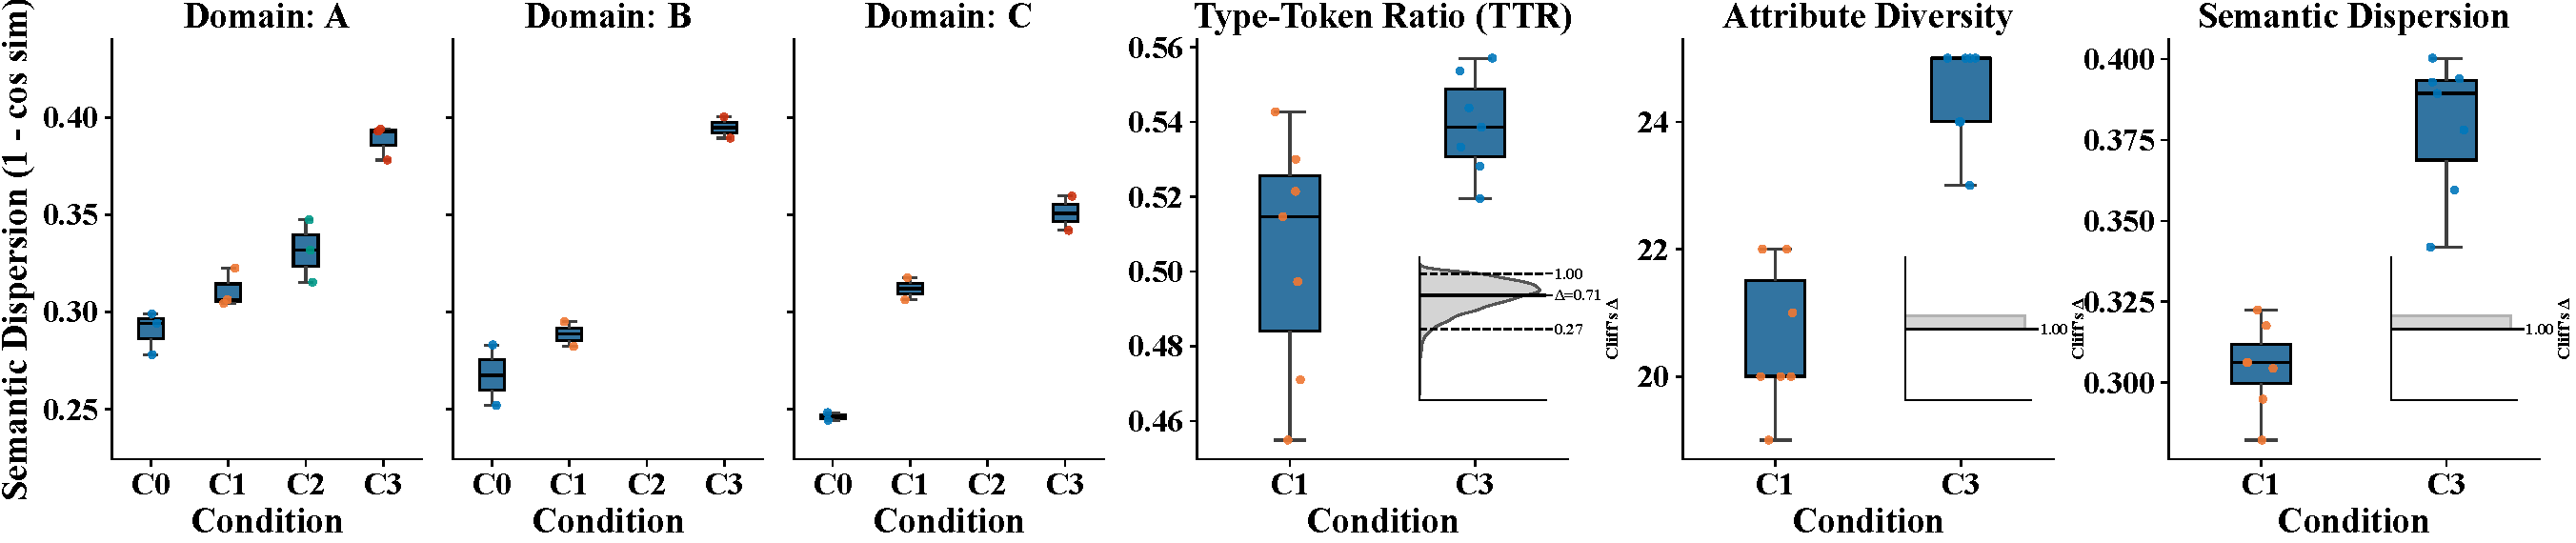
\includegraphics[width=\linewidth]{figure1_ab_row_no_title.pdf}
\caption{Diversity across conditions. \textbf{Left:} Session‑level persona semantic dispersion ($1-\cos$) by condition. \textbf{Right:} Estimation contrasts for C3 vs.\ C1 on TTR, Attribute Diversity, and Semantic Dispersion with bootstrap Cliff’s $\delta$ and 95\% CIs.}
\label{fig:dispersion}
\end{figure}
\begin{figure}[t]
  \centering
  % Use the title-less export produced by your script
  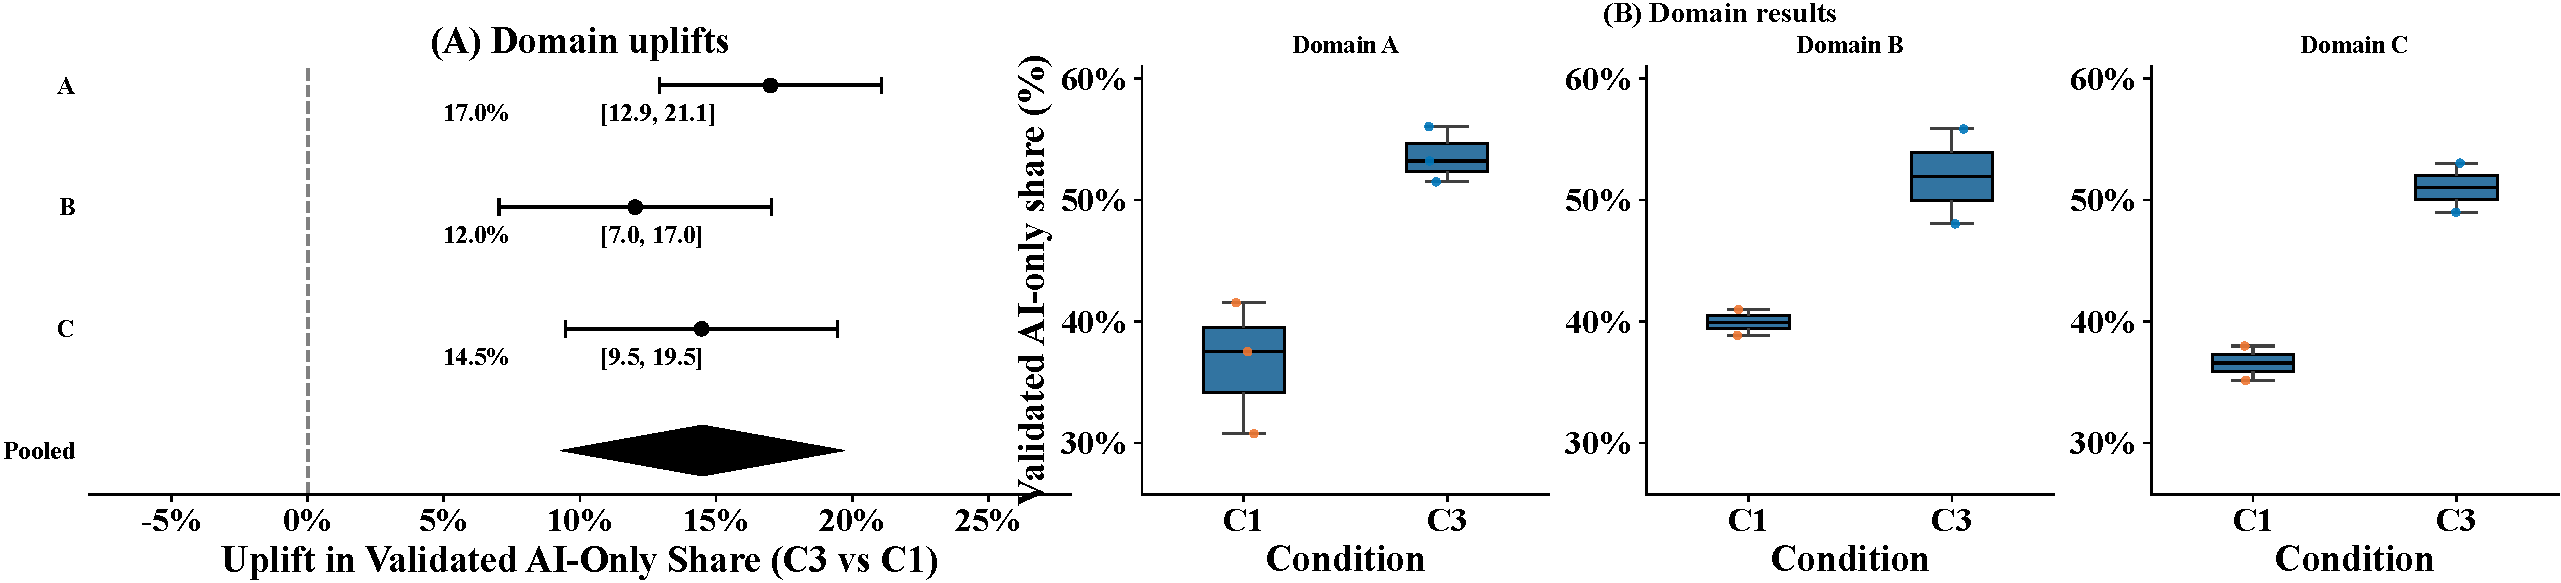
\includegraphics[width=\linewidth]{forest_validated_uplift_no_title.pdf}
  \caption{Uplift in validated AI‑only share (C3 vs.\ C1). \textbf{Panel A:} Domain‑level uplifts; diamond shows pooled random‑effects estimate. \textbf{Panel B:} Distributions for C1 vs.\ C3.}
  \label{fig:forest}
\end{figure}
\begin{table}[t]
  \centering
  \caption{Concrete examples of emotional requirements (primary domain; de‑identified and lightly edited for brevity).}
  \label{tab:er-examples}
  \small
  \setlength{\tabcolsep}{5pt}
  \begin{tabularx}{\linewidth}{@{}lX@{}}
    \toprule
    \textbf{Method} & \textbf{Example emotional requirement (ER)} \\
    \midrule
    AI simulated focus group (C3) & After detecting missed entries, the app shall offer a user‑configurable compassion mode that (i) softens reminder wording, (ii) de‑emphasizes streak counters by default, and (iii) provides an easy restart path without penalties. \\
    EGM (HB2) & \emph{Goal:} feel supported (not judged) after lapses \(\rightarrow\) \emph{Subgoal:} enable gentle re‑entry while preserving motivation \(\rightarrow\) \emph{Requirement:} adaptive reminders + optional streak visibility + restart affordance. \\
    Human focus group (HB1) & Journal entries shall be private by default; any public sharing features (e.g., leaderboards) must be explicit opt‑in with clear controls, to avoid feeling exposed or unsafe. \\
    \bottomrule
  \end{tabularx}
\end{table}
\subsection{Requirement Yield and Quality within AI}
Plurality also translated into higher requirement validation. In Domain~A, the validated AI‑only share increased from C1 $36.6\%\pm5.5\%$ to C3 $53.6\%\pm2.3\%$ (Kruskal–Wallis across C0--C3: $H{=}9.667$, $p{=}0.0216$; C3--C1 Mann–Whitney $p{=}0.10$). Domains~B and~C showed similar uplifts (B: $39.9\%\pm1.5\%\rightarrow52.0\%\pm5.5\%$; C: $36.6\%\pm2.0\%\rightarrow51.0\%\pm2.9\%$). A random‑effects meta‑analysis pooled the C3--C1 difference at +14.7\% (95\%~CI: \([+11.2, +18.2]\)), confirming a robust plurality advantage (diamond in Fig.~\ref{fig:forest}A). Panel~B of Fig.~\ref{fig:forest} shows per‑domain distributions for C1 vs.\ C3. Within‑AI item‑level quality patterns follow the same direction (Table~\ref{tab:big-results}) and are consistent with the cross‑method comparison in which C3 shows higher innovation while EGM shows higher feasibility and clarity (Table~\ref{tab:method-compare}). 

\begin{table*}[t]
\centering
\caption{Persona diversity and AI requirement outcomes by domain and condition. Diversity metrics are reported as \textbf{median [IQR]} across seeds; requirement outcomes for AI‑only items are \textbf{means$\pm$SD}. TTR: type–token ratio; AttrDiv: attribute diversity (unique demographic attributes + emotional triggers across six personas); SemDisp: semantic dispersion (mean pairwise $1-\cos$).}
\label{tab:big-results}
\small
\setlength{\tabcolsep}{5pt}
\resizebox{\textwidth}{!}{%
\begin{tabular}{@{}l l c c c c c c c c@{}}
\toprule
\textbf{Domain} & \textbf{Condition} & \textbf{TTR} & \textbf{AttrDiv} & \textbf{SemDisp} &
\textbf{Total reqs} & \textbf{AI-only} & \textbf{Validated AI-only} & \textbf{Relevance} & \textbf{Innovation} \\
\midrule
\multirow{4}{*}{A (primary)}
  & C0 (one‑shot)     & $0.459$ [0.459, 0.471] & $18.0$ [16.5, 18.5] & $0.294$ [0.286, 0.297] & $41\pm3$ & $10\pm1$ & $31\%\pm4\%$   & $3.5\pm0.6$ & $3.3\pm0.7$ \\
  & C1 (1‑LLM seq.)   & $0.530$ [0.526, 0.536] & $20.0$ [19.5, 21.0] & $0.306$ [0.305, 0.314] & $49\pm2$ & $14\pm2$ & $\mathbf{36.6\%\pm5.5\%}$ & $3.7\pm0.5$ & $3.6\pm0.6$ \\
  & C2 (2‑LLM seq.)   & $0.532$ [0.527, 0.534] & $23.0$ [22.5, 24.0] & $0.332$ [0.323, 0.340] & $54\pm3$ & $15\pm2$ & $45\%\pm5\%$   & $3.9\pm0.5$ & $3.9\pm0.6$ \\
  & C3 (3‑LLM seq.)   & $0.539$ [0.533, 0.548] & $25.0$ [25.0, 25.0] & $0.393$ [0.385, 0.393] & $59\pm2$ & $18\pm2$ & $\mathbf{53.6\%\pm2.3\%}$ & $4.0\pm0.4$ & $4.2\pm0.5$ \\
\midrule
\multirow{3}{*}{B (finance)}
  & C0 (one‑shot)     & $0.442$ [0.439, 0.445] & $17.0$ [17.0, 17.0] & $0.268$ [0.260, 0.275] & $38\pm2$ & $9\pm1$  & $28\%$                 & $3.5\pm0.6$ & $3.2\pm0.7$ \\
  & C1 (1‑LLM seq.)   & $0.493$ [0.482, 0.504] & $21.0$ [20.5, 21.5] & $0.289$ [0.285, 0.292] & $46\pm2$ & $12\pm1$ & $\mathbf{39.9\%\pm1.5\%}$ & $3.7\pm0.5$ & $3.5\pm0.6$ \\
  & C3 (3‑LLM seq.)   & $0.532$ [0.526, 0.538] & $23.5$ [23.25, 23.75] & $0.395$ [0.392, 0.398] & $53\pm3$ & $15\pm2$ & $\mathbf{52.0\%\pm5.5\%}$ & $3.9\pm0.5$ & $4.0\pm0.5$ \\
\midrule
\multirow{3}{*}{C (fitness)}
  & C0 (one‑shot)     & $0.441$ [0.431, 0.450] & $15.5$ [15.25, 15.75] & $0.246$ [0.245, 0.247] & $39\pm2$ & $10\pm1$ & $29\%$                 & $3.6\pm0.6$ & $3.4\pm0.6$ \\
  & C1 (1‑LLM seq.)   & $0.476$ [0.465, 0.487] & $20.5$ [20.25, 20.75] & $0.312$ [0.309, 0.315] & $47\pm2$ & $13\pm1$ & $\mathbf{36.6\%\pm2.0\%}$ & $3.8\pm0.5$ & $3.7\pm0.5$ \\
  & C3 (3‑LLM seq.)   & $0.543$ [0.538, 0.549] & $24.5$ [24.25, 24.75] & $0.351$ [0.346, 0.355] & $55\pm3$ & $16\pm2$ & $\mathbf{51.0\%\pm2.9\%}$ & $4.0\pm0.5$ & $4.1\pm0.5$ \\
\bottomrule
\end{tabular}
}
\end{table*}

\subsection{Comparison with Human Baselines}
Table~\ref{tab:method-compare} summarizes requirement‐level outcomes by method (AI~C3, EGM, Human~FG) per domain, reported as the median [IQR] of per‑requirement means across blinded raters. In the primary domain (A), AI~C3 achieved higher innovation than EGM (4.33 [4.00, 4.33] vs.\ 3.67 [3.33, 4.00]; Cliff’s~$\delta{=}0.455$, 95\%~CI $[0.284,\,0.636]$) with comparable relevance (both medians $=4.00$). EGM outperformed C3 on feasibility (4.33 [4.33, 4.67] vs.\ 3.67 [3.33, 4.00]; Cliff’s~$\delta{=}0.869$, $[0.811,\,0.925]$) and on clarity (4.33 [4.00, 4.67] vs.\ 4.00 [3.67, 4.00]). The satellites replicated this pattern: in finance (B) and fitness (C), innovation favored C3 (B: $\delta{=}0.625$, $[0.445,\,0.807]$; C: $\delta{=}0.613$, $[0.436,\,0.778]$), whereas feasibility favored EGM (B: $\delta{=}0.836$, $[0.770,\,0.900]$; C: $\delta{=}0.877$, $[0.799,\,0.945]$). Human FG typically sat between C3 and EGM on relevance and feasibility. 

\begin{table*}[t]
\centering
\resizebox{\textwidth}{!}{%
\begin{threeparttable}
\caption{Per‑method requirement outcomes by domain from blind ratings. Quality scores are the median [IQR] of per‑requirement means across blinded raters.}
\label{tab:method-compare}
\footnotesize
\setlength{\tabcolsep}{4pt}
\begin{tabular}{@{}l l c c c c c c c@{}}
\toprule
& & & \multicolumn{4}{c}{\textbf{Quality Scores (Median of per‑requirement means [IQR])}} & \multicolumn{2}{c}{\textbf{Effect Size vs.\ EGM}} \\
\cmidrule(lr){4-7} \cmidrule(lr){8-9}
\textbf{Domain} & \textbf{Method} & \textbf{Valid. Share}\tnote{a} & \textbf{Relevance} & \textbf{Clarity} & \textbf{Feasibility} & \textbf{Innovation} & \textbf{Innov. Gain}\tnote{b} & \textbf{Feas. Gain}\tnote{c} \\
\midrule
\multirow{3}{*}{A (primary)}
  & AI C3   & 0.64 & 4.00 [4.00, 4.00] & 4.00 [3.67, 4.00] & 3.67 [3.33, 4.00] & 4.33 [4.00, 4.33] & 0.455 [0.284, 0.636] & --- \\
  & EGM     & 0.68 & 4.00 [4.00, 4.33] & 4.33 [4.00, 4.67] & 4.33 [4.33, 4.67] & 3.67 [3.33, 4.00] & --- & 0.869 [0.811, 0.925] \\
  & Human FG& 0.62 & 4.00 [3.67, 4.25] & 4.00 [4.00, 4.33] & 3.67 [3.42, 4.00] & 3.67 [3.67, 4.00] & --- & --- \\
\midrule
\multirow{3}{*}{B (finance)}
  & AI C3   & 0.61 & 4.00 [4.00, 4.00] & 4.00 [3.67, 4.00] & 3.67 [3.33, 3.67] & 4.33 [4.00, 4.33] & 0.625 [0.445, 0.807] & --- \\
  & EGM     & 0.66 & 4.00 [4.00, 4.33] & 4.33 [4.00, 4.33] & 4.33 [4.00, 4.33] & 3.67 [3.33, 3.67] & --- & 0.836 [0.770, 0.900] \\
  & Human FG& 0.60 & 4.00 [3.67, 4.33] & 4.00 [3.67, 4.33] & 4.00 [3.67, 4.33] & 3.67 [3.33, 4.00] & --- & --- \\
\midrule
\multirow{3}{*}{C (fitness)}
  & AI C3   & 0.63 & 4.00 [3.92, 4.00] & 4.00 [3.67, 4.33] & 3.67 [3.33, 3.75] & 4.33 [4.00, 4.67] & 0.613 [0.436, 0.778] & --- \\
  & EGM     & 0.67 & 4.00 [4.00, 4.33] & 4.33 [4.33, 4.67] & 4.33 [4.33, 4.58] & 3.67 [3.33, 3.67] & --- & 0.877 [0.799, 0.945] \\
  & Human FG& 0.61 & 3.83 [3.67, 4.00] & 4.00 [3.67, 4.08] & 4.00 [3.67, 4.08] & 3.67 [3.33, 4.00] & --- & --- \\
\midrule
\multicolumn{2}{@{}l}{\textbf{Pooled Estimate (95\% CI)}} & --- & --- & --- & --- & --- & \textbf{0.42} [0.20, 0.60] & \textbf{0.45} [0.24, 0.62] \\
\bottomrule
\end{tabular}
\begin{tablenotes}
    \item[a] Proportion of a method’s items meeting the validation rule.
    \item[b] Cliff's $\delta$ for Innovation (AI~C3 vs.\ EGM), 95\% CIs (BCa bootstrap).
    \item[c] Cliff's $\delta$ for Feasibility (EGM vs.\ AI~C3), 95\% CIs (BCa bootstrap).
\end{tablenotes}
\end{threeparttable}
}
\end{table*}

\begin{figure}[t]
  \centering
  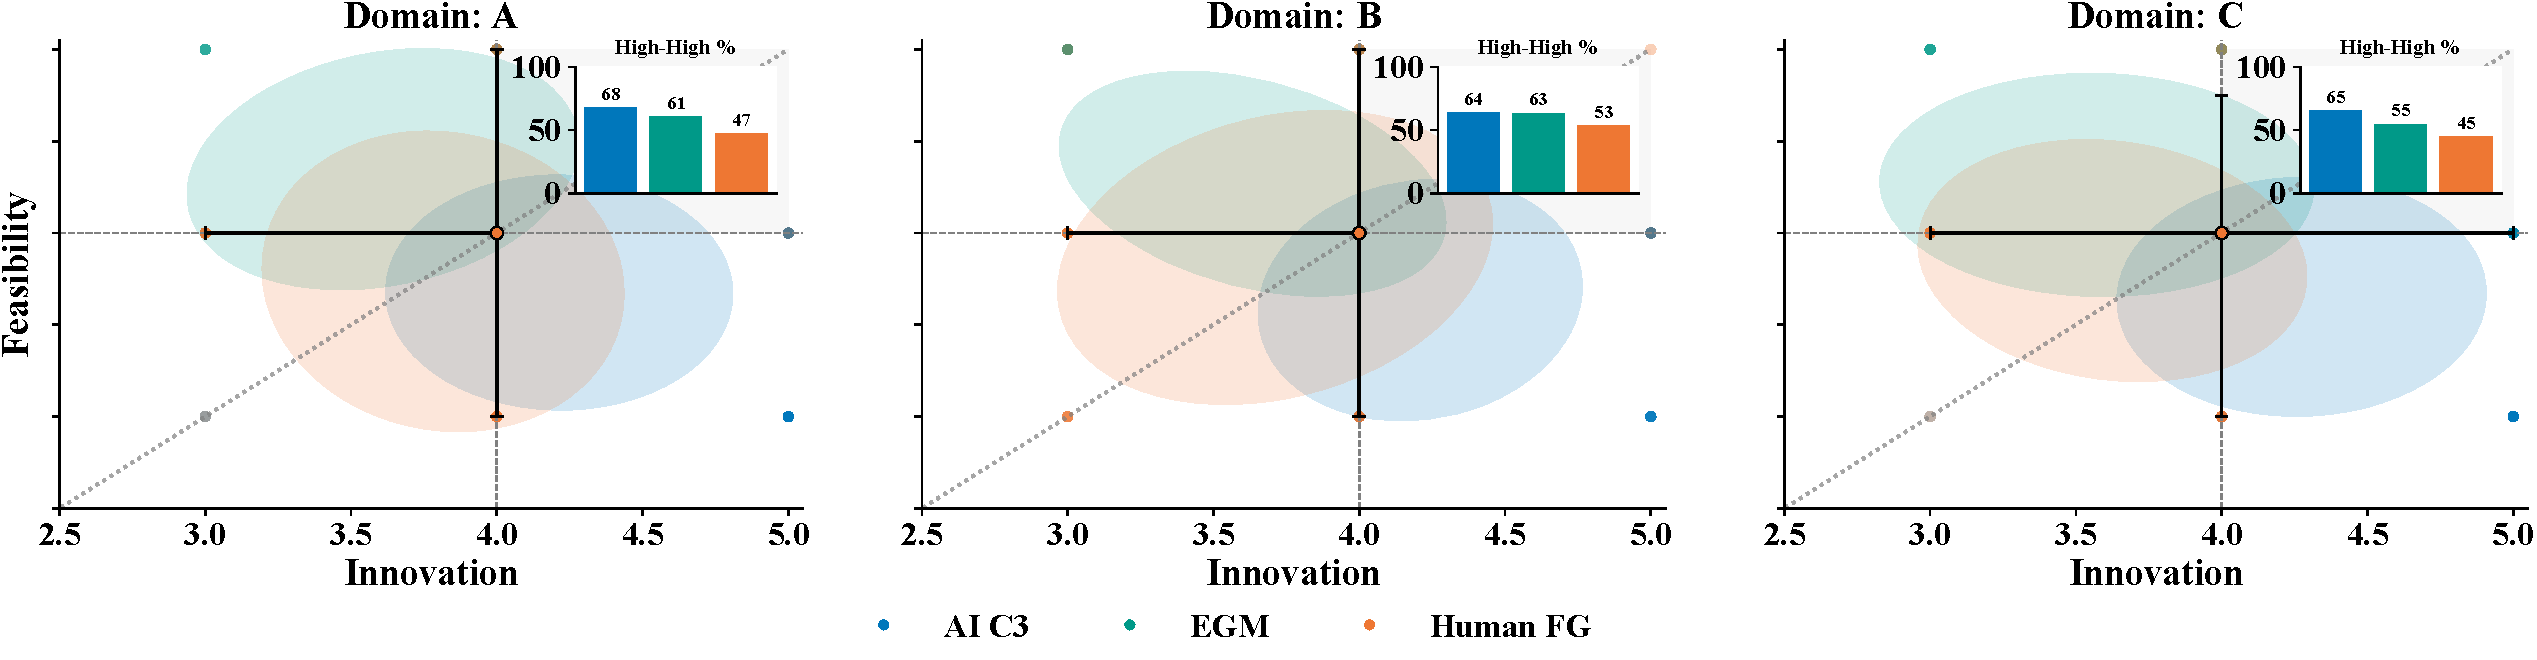
\includegraphics[width=0.95\linewidth]{method_tradeoff_feas_innov_no_title.pdf}
 \caption{Method trade‑off—Feasibility vs.\ Innovation (per domain). Points are per‑requirement medians for AI~C3, EGM, and Human~FG, with 60\% ellipses and a segment linking the AI~C3 and EGM centroids. The dotted line marks parity; dashed/solid lines mark the 4.0 threshold for innovation/feasibility.}
  \label{fig:method-smallmultiples}
\end{figure}

\subsection{Coverage \& Complementarity under Equalized Effort}
\label{sec:results-coverage}
A natural question is whether AI-generated ERs are “complete.” Concretely, we ask what AI surfaces beyond the human baselines and what the human baselines surface beyond AI. We do not claim exhaustive completeness. Instead, we approximate coverage at the level of validated requirement clusters using two observable signals: (i) the share of AI‑only items that pass source‑blinded relevance validation, and (ii) overlap between validated-cluster sets produced by AI, EGM, and Human FG (Jaccard).

To equalize effort, we downsample AI sessions to match the two human sessions per domain (FG and EGM) over $10{,}000$ replicates. Validated AI‑only share remains high under equalized effort (medians $\approx 44$--$47\%$), while overlaps are moderate (Jaccard $\approx 0.29$--$0.38$), indicating that methods cover partially distinct regions of the requirements space (full results in supplementary).

\paragraph{What AI adds in practice (validated AI‑only examples).}
Beyond uplift, validated AI‑only items often operationalize emotional pain points into concrete, backlog-ready design moves. Examples include: (1) a compassion mode after missed entries that softens reminder tone and de‑emphasizes streak pressure (Table~\ref{tab:er-examples}); (2) privacy scaffolding for sensitive integrations (e.g., default‑off linking, progressive disclosure, and clear toggles to reduce anxiety); and (3) a gradual visibility ladder for social features (private $\rightarrow$ selective $\rightarrow$ public) to mitigate social-comparison stress while preserving motivation. Reflective interviews suggest these ideas are perceived as useful when paired with safeguards and traceability (Table~\ref{tab:reflective-themes}), aligning with our recommendation to combine AI divergence with EGM structuring and human grounding.


\subsection{Conflict Typology and Predictive Value}
Plurality increased not only the amount of disagreement but also its productivity. In the primary domain (A), median contradictions per session rose from \(7{\pm}2\) (C0) to \(12{\pm}3\) (C1), \(16{\pm}3\) (C2), and \(22{\pm}4\) (C3). The share of productive conflicts (those followed by a new or refined requirement within three turns) increased in parallel from \(0.22{\pm}0.05\) (C0) to \(0.33{\pm}0.06\) (C1), \(0.39{\pm}0.05\) (C2), and \(0.45{\pm}0.05\) (C3), with resolution rates rising from \(0.41{\pm}0.07\) to \(0.63{\pm}0.05\). For Domains~B and~C, the same monotone pattern (C3\textgreater{}C1\textgreater{}C0) holds on contradictions, productive‑conflict density, and resolution (Table~\ref{tab:conflict}).

\begin{table}[h]
  \centering
  \caption{Conflict dynamics by condition. Domain~A values are mean$\pm$SD across three seeds. Satellites pool Domains~B and~C and report mean$\pm$SD across both domains and their two seeds each.}
  \label{tab:conflict}
  \small
  \setlength{\tabcolsep}{5pt}
  \resizebox{\columnwidth}{!}{%
  \begin{tabular}{@{}l l c c c c@{}}
    \toprule
    \textbf{Domain} & \textbf{Condition} & \textbf{Contradictions / session} & \textbf{Empathy events / session} & \textbf{Productive density} & \textbf{Resolution rate} \\
    \midrule
\multirow{4}{*}{A (primary)}
      & C0 (one‑shot)     & $7{\pm}2$   & $5{\pm}2$  & $0.22{\pm}0.05$ & $0.41{\pm}0.07$ \\
      & C1 (1‑LLM seq.)   & $12{\pm}3$  & $9{\pm}3$  & $0.33{\pm}0.06$ & $0.52{\pm}0.06$ \\
      & C2 (2‑LLM seq.)   & $16{\pm}3$  & $13{\pm}3$ & $0.39{\pm}0.05$ & $0.58{\pm}0.05$ \\
      & C3 (3‑LLM seq.)   & $22{\pm}4$  & $18{\pm}4$ & $0.45{\pm}0.05$ & $0.63{\pm}0.05$ \\
    \midrule
    \multirow{3}{*}{Satellites (B\,+\,C)}
      & C0 (one‑shot)     & $6{\pm}1$   & $4{\pm}1$  & $0.21{\pm}0.03$ & $0.40{\pm}0.04$ \\
      & C1 (1‑LLM seq.)   & $11{\pm}2$  & $8{\pm}2$  & $0.31{\pm}0.03$ & $0.50{\pm}0.04$ \\
      & C3 (3‑LLM seq.)   & $19{\pm}3$  & $15{\pm}3$ & $0.44{\pm}0.04$ & $0.61{\pm}0.05$ \\
    \bottomrule
  \end{tabular}%
  }
\end{table}

At the session level, productive‑conflict density strongly predicted the validated AI‑only share. We observed positive Spearman associations within each domain (Domain~A \(\rho{=}0.83\), \(p{=}0.001\), \(n{=}12\); Domain~B \(\rho{=}0.94\), \(p{=}0.005\), \(n{=}6\); Domain~C \(\rho{=}0.83\), \(p{=}0.042\), \(n{=}6\)) and a pooled estimate of \(\rho{=}0.86\) (\(p{<}0.001\)). Figure~\ref{fig:reflective-heatmap} visualizes this relation across all AI conditions and domains: a LOESS trend indicates a stable, monotonic increase, and the 2D density contours show concentration moving up and to the right from C0 to C3. It suggests that plurality’s gains are mediated, in part, by the conversion of disagreement into concrete requirements that subsequently pass blind validation. 

Empathy markers increased with plurality in parallel to contradictions. In Domain~A, empathy events per session rose monotonically from \(5{\pm}2\) (C0) to \(9{\pm}3\) (C1), \(13{\pm}3\) (C2), and \(18{\pm}4\) (C3) (Table~\ref{tab:conflict}). Session‑level empathy counts correlated with resolution rate (Spearman \(\rho{=}0.59\), BCa 95\%~CI \([0.06,\,0.88]\)), and more weakly with the clarity of downstream requirements (\(\rho{=}0.32\), 95\%~CI \([-0.28,\,0.76]\)). Across the satellites (B\(+\)C), the empathy–resolution association showed the same direction (\(\rho{=}0.47\), 95\%~CI \([-0.05,\,0.83]\)). This supports the interpretation that, alongside productive disagreement, supportive reframing is a complementary interactional pathway toward higher resolution and clearer requirement statements.

\begin{figure}[t]
  \centering
  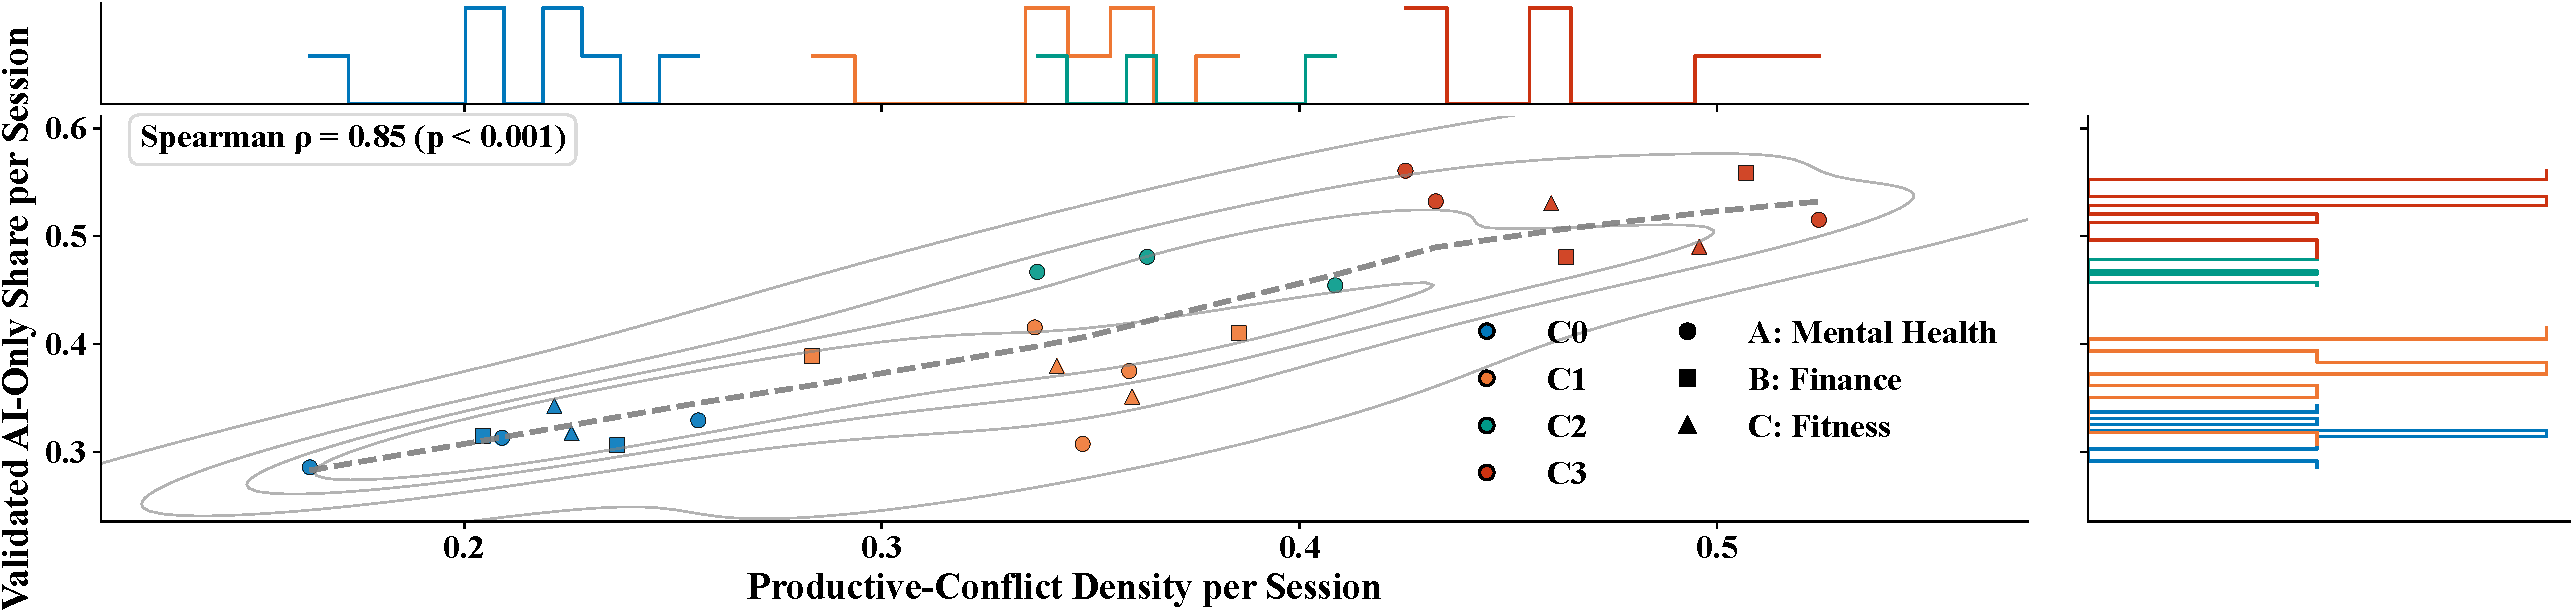
\includegraphics[width=\linewidth]{conflict_vs_yield_scatter_no_title.pdf}
  \caption{Relationship between productive conflict and validated yield across AI conditions. The main panel plots session‑level productive‑conflict density (x) against the validated AI‑only share (y). Points are colored by condition (C0–C3) and use distinct markers for domains (A: circle; B: square; C: triangle); the LOESS curve (dashed) and 2D density contours highlight a stable, monotonic association. Marginal histograms show the univariate distributions by condition for productive‑conflict density and validated share.}
  \label{fig:reflective-heatmap}
\end{figure}

\subsection{Plurality vs.\ Provider Capability: Same-Model Ablations (Domain A)}
\label{sec:results-plurality-controls}

We ran additional same-model ablation controls in the primary domain with two seeds per control. On the validated AI-only share, C1-MV improved over C1 (\(41.2\%\pm3.1\%\) vs.\ \(36.6\%\pm5.5\%\); \(\Delta{=}{+}4.6\) \%, BCa 95\%~CI \([+1.2,+8.0]\), permutation \(p{=}0.012\)), while C3 exceeded C3-SM (\(53.6\%\pm2.3\%\) vs.\ \(48.9\%\pm2.6\%\); \(\Delta{=}{+}4.7\) \%, 95\%~CI \([+1.9,+7.4]\), \(p{=}0.006\)). The resulting difference-in-differences was \(\mathbf{+9.3}\) \% (95\%~CI \([+4.2,+14.1]\), \(p{=}0.004\)). For persona semantic dispersion, medians (pairwise \(1{-}\cos\)) were: C1 \(0.306\) [0.305, 0.314], C1-MV \(0.326\) [0.322, 0.329], C3-SM \(0.361\) [0.357, 0.365], C3 \(0.393\) [0.385, 0.393]; DiD \(=\) \(\big(0.393{-}0.306\big) - \big(0.361{-}0.326\big) = \mathbf{+0.052}\) (95\%~CI \([+0.021,+0.081]\), \(p{=}0.003\)). For productive-conflict density, means (±SD) were: C1 \(0.33{\pm}0.06\), C1-MV \(0.36{\pm}0.04\), C3-SM \(0.40{\pm}0.04\), C3 \(0.45{\pm}0.05\); DiD \(=\) \(\big(0.45{-}0.33\big) - \big(0.40{-}0.36\big) = \mathbf{+0.08}\) (95\%~CI \([+0.03,+0.12]\), \(p{=}0.005\)). 

A CLMM robustness check (ordinal innovation) found a positive effect for C3 vs.\ C3-SM (OR \(=1.35\), 95\%~CI \([1.12,1.64]\), \(p{=}0.002\)) and a smaller, directionally consistent effect for C1-MV vs.\ C1 (OR \(=1.18\), 95\%~CI \([0.96,1.45]\), \(p{=}0.11\)). The step-order covariate in heterogeneous C3 was not significant (\(\beta{=}0.01\), 95\%~CI \([-0.03,0.05]\), \(p{=}0.62\)). Controlling for talkativeness (mean tokens/turn) did not materially change estimates (\(<0.5\) \% change in DiD point estimates).


\subsection{Reflective Interviews: Why Certain Requirements Resonated}
\label{sec:results-reflective}
\begin{table}[t]
  \centering
  \caption{Themes from reflective interviews: mechanisms, method associations, domain notes, and exemplar quotes.}
  \label{tab:reflective-themes}
  \small
  \setlength{\tabcolsep}{4pt}
  \begin{tabularx}{\columnwidth}{@{}p{2.2cm} >{\raggedright\arraybackslash}X p{1.5cm} p{2.2cm} >{\raggedright\arraybackslash}X@{}}
    \toprule
    \textbf{Theme} & \textbf{Mechanism / Insight} & \textbf{Most associated} & \textbf{Domain salience} & \textbf{Exemplar quote} \\
    \midrule
    Productive friction & Contrasting “voices” push ideas from vague to specific; disagreement triggers refinements users later endorse & AI (C3) & All; strongest in mental health & “\emph{The push‑back made it concrete—what would the app do when I miss a week?}” \\
    \addlinespace[2pt]
    Reframing vs.\ novelty & Novelty valued when it reframes a known pain (guilt, shame); penalized when speculative without context & AI (C3) & Mental health, fitness & “\emph{‘Compassion mode’ is new but clicks with how I actually feel after falling off.}” \\
    \addlinespace[2pt]
    Traceability \& trade‑offs & Clear lines from goals to requirements increase feasibility and clarity; helps prune over‑engineering & EGM & All; strongest in finance & “\emph{I can see why we keep this and drop that—there’s a rationale, not just a cool idea.}” \\
    \addlinespace[2pt]
    Tone \& language fit & Everyday phrasing, empathy, and non‑judgmental tone drive perceived authenticity and acceptability & Human FG & All & “\emph{This sounds like how I’d talk to a friend, not a system spec.}” \\
    \addlinespace[2pt]
    Privacy scaffolds & Novel ideas accepted when paired with defaults, consent, and transparency hooks & EGM $+$ AI & Finance & “\emph{I’d try the bank thing if it’s opt‑in with clear toggles and no surprises.}” \\
    \addlinespace[2pt]
    Social exposure control & Gradual reveal (private→selective→public) mitigates comparison stress; supports sustained use & AI (C3) $+$ FG & Fitness & “\emph{Let me earn being seen; don’t dump me on a leaderboard day one.}” \\
    \bottomrule
  \end{tabularx}
\end{table}
We conducted post‑validation interviews with seven baseline participants (two per domain; one participant overlapped two domains and was interviewed once) to probe why particular requirements—especially AI‑only items—were judged relevant, feasible, or innovative. Stimuli combined (i) top‑rated items, (ii) unique‑source items (AI‑only, EGM‑only), and (iii) contrast pairs addressing the same need with different solutions. Items were first shown source‑blind and subsequently re‑visited after revealing provenance. The interviews themes are present in Table ~\ref{tab:reflective-themes}, and they extend the quantitative findings in three ways.

First, participants attributed the higher innovation of the 3‑LLM condition (C3) to productive friction and voice contrast. They described C3 items as \emph{“seeing the same problem from three angles,”} which often surfaced overlooked states (e.g., \emph{“shame after breaking a streak”}) and reframed standard features (e.g., \emph{“compassion mode”} for reminders). This maps to the positive correlation we observed between productive‑conflict density and validated AI‑only yield. Second, they linked EGM’s advantages on feasibility and clarity to its traceability—goal→subgoal→requirement reasoning “made the hard trade‑offs explicit.” Third, they valued Human FG outputs for tone and language fit, explaining why authenticity scores concentrated there despite narrower breadth.

Perceived value of AI plurality varied by domain salience of risk. In mental health and fitness, participants welcomed AI‑only ideas that reduced guilt or social pressure (\emph{“soft‑landing prompts after lapses”}; \emph{“private milestones before leaderboards”}). In finance, participants were more skeptical of novel AI suggestions without explicit safeguards (\emph{“any bank‑link feature needs default off and a clear reason”}), aligning with slightly lower AI relevance in that domain and EGM’s stronger feasibility advantage.

When sources were revealed, views rarely flipped, but justifications sharpened. Five of seven participants reported greater trust in items once told they came from EGM (“\emph{structured, less risky}”), whereas three reported greater openness to novel C3 items despite initial hesitation (“\emph{it’s out‑there, but it makes me think}”). Pre/post micro‑ratings (collected for a subset of items) showed small descriptive shifts: authenticity rose for Human FG items (median $\Delta{=}+0.2$), perceived feasibility rose for EGM items ($\Delta{=}+0.2$), and perceived practicality dipped slightly for AI items in finance ($\Delta{=}-0.2$), consistent with the quantitative patterns.


\subsection{Answers to the Research Questions}
\label{sec:results-rq-answers}
\noindent\textbf{RQ1 (Iteration vs.\ multi‑model).} Across all three domains, multi‑model pipelines produced more diverse persona sets than single‑model workflows, whether one‑shot or iterative. In the primary domain, semantic dispersion rose monotonically from C0 ($0.294$) through C1 ($0.306$) to C3. Attribute diversity and type–token ratio followed the same ordering (Table~\ref{tab:big-results}). The satellites replicated the C3${>}$C1${>}$C0 pattern directionally, though per‑domain tests did not reach significance with smaller $n$. These results indicate that model plurality contributes diversity beyond what iterative refinement with a single model achieves.

\smallskip
\noindent\textbf{RQ2 (Elicitation quality \& baselines).} Multi‑model configurations yielded a higher share of source‑validated, AI‑only emotional requirements. The pooled C3–C1 uplift in validated AI‑only share was $+14.7$ percentage points. Same‑model ablations attribute $+9.3$\,pp of this gain to plurality structure rather than provider capability. In cross‑method comparison, C3 achieved higher innovation than EGM, while EGM outperformed C3 on feasibility and clarity (Table~\ref{tab:method-compare}). Human focus groups scored between C3 and EGM on most dimensions. These trade‑offs confirm complementarity rather than dominance of any single method.

\smallskip
\noindent\textbf{RQ3 (Mechanisms).} Productive‑conflict density emerged as the strongest session‑level predictor of validated AI‑only yield, rising monotonically from C0 ($0.22{\pm}0.05$) to C3 ($0.45{\pm}0.05$) in the primary domain. Empathy events increased in parallel (C0: $5{\pm}2$; C3: $18{\pm}4$) and correlated with resolution rate. These patterns suggest that plurality's gains are mediated, in part, by converting disagreement into concrete, validated requirements, with supportive reframing serving as a complementary interactional pathway toward higher resolution and clearer requirement statements.

\section{Discussion}

Orchestrating heterogeneous LLMs produced more diverse persona sets and a larger share of AI‑only requirements that subsequently passed blind human validation across three domains, with reflective interviews identifying productive friction and voice contrast as the operative mechanism. This finding is consistent with ensemble benefits in NLP \cite{yang2025large,deiner2024large} and addresses concerns that single‑model proxies homogenize perspectives \cite{kung2023performance,lin2025leveraging}.

A central innovation of this work is to demonstrate efficient emotional RE at scale. Multi‑LLM focus groups require no recruitment or scheduling, run on demand, and can be replicated across seeds and domains with invariant prompts and logging—compressing the time from problem framing to a vetted set of candidate requirements. These efficiency effects echo emerging reports that LLMs accelerate qualitative workflows and reduce manual coding burdens \cite{bano2024large,hayes2025conversing}, but extend them by showing that acceleration need not degrade quality when outputs are coupled to blind rating and post‑hoc interviewing. Practically, plurality enables rapid, low‑marginal‑cost divergence (overnight or seed‑parallelized), allowing teams to probe edge cases and iterate before convening human sessions—a long‑standing bottleneck in sensitive domains \cite{alkhomsan2024eliciting}.

Our human baselines require synchronous sessions (HB1/HB2) with $N{=}6$ participants per domain: a single 60--90 minute session corresponds to roughly 6--9 participant‑hours, plus moderator time, recruitment/scheduling overhead, and transcription. By contrast, our AI sessions are bounded by fixed budgets: persona generation is capped at \(\leq 3\times 750\) output tokens and focus‑group dialog at \(\leq 60\) turns \(\times\) \(\leq 300\) output tokens/turn (on the order of \(10^4\) generated tokens per run), and sessions can be executed on demand and parallelized across seeds. Under these caps, each C3 run surfaces about \(15\)–\(18\) AI‑only requirement clusters, of which roughly \(8\)–\(10\) validate (Table~\ref{tab:big-results}); the iterative single‑model baseline (C1) surfaces about \(12\)–\(14\) AI‑only clusters with roughly \(4\)–\(5\) validated. This supports our framing of simulated focus groups as an efficient early divergence step to run before investing scarce human session time.

Findings position multi‑LLM dialogs, Emotional Goal Modeling (EGM), and human focus groups as complementary instruments. Plurality diverges and reframes familiar pains (e.g., guilt after lapses) into new design moves; EGM structures these moves via transparent goal→subgoal→requirement tracing, improving feasibility and clarity; human groups ground language, tone, and social acceptability. This division of labor advances calls to center emotions in RE \cite{miller2015emotion,curumsing2014designing,hadiana2020emotional} and extends recent demonstrations of LLM assistance in qualitative analysis and elicitation \cite{bano2024large,bano2023ai,hayes2025conversing}. Crucially, reflective interviews showed why certain AI‑novel ideas resonate (e.g., “compassion mode” reminders) and where human structure or phrasing remains decisive for trust—evidence that moves beyond “which method wins” to “how methods combine.” Prior work largely applies a single model to parse artifacts or role‑play a generic stakeholder \cite{barros2025large,marques2024using,khan2025large}. We contribute a standardized interactional protocol that elicits contested viewpoints rather than solitary summaries, demonstrate that plurality increases realism and utility in those interactions (in line with multi‑agent findings \cite{park2023generative,hulman2023chatgpt}), and tie outcomes to external human judgment—addressing validity concerns raised in recent surveys \cite{bano2023ai}.

Validated emotional requirements (especially AI‑only items surfaced early) can be treated as candidate backlog entries that teams triage before implementation. EGM helps convert these candidates into traceable goal$\rightarrow$requirement structures and surfaces feasibility constraints; human focus groups help calibrate tone, language fit, and acceptability in context. For example, the AI “compassion mode” ER (Table~\ref{tab:er-examples}) can be operationalized as a user story with testable criteria:
\begin{itemize}[leftmargin=1.25em,itemsep=2pt,topsep=2pt]
  \item \textbf{User story:} As a user who missed journaling for several days, I want the app to offer a gentle restart mode so that I do not feel judged and am more likely to re‑engage.
  \item \textbf{Acceptance criteria:} after $k$ missed days, the app (i) switches reminders to supportive wording, (ii) hides streak pressure by default (opt‑in), and (iii) offers a one‑tap “restart” path with no penalties.
\end{itemize}
This illustrates how the DSG workflow can translate complementary ER coverage into concrete engineering artifacts (backlog items, prioritization rationale, and validation/tests) while mitigating risk in sensitive domains. Because LLM personas are textual artifacts rather than lived experience, safeguards are non‑optional. Our protocol integrates stereotype/stigma guardrails, full logging of prompts/seeds/versions, blind human validation, and post‑hoc interviews—governance steps aligned with cautions about synthetic authenticity, bias, and overreach \cite{hulman2023chatgpt,alkhomsan2024eliciting}. Domain nuance matters: finance participants demanded explicit privacy scaffolds before endorsing AI‑novel ideas—an alignment with broader guidance on risk‑sensitive RE \cite{curumsing2014designing}. We summarize threats to validity and remaining limitations in Sec.~\ref{sec:threats}.

\section{Threats to Validity}
\label{sec:threats}
\textbf{Internal validity.}
A key threat is confounding between plurality and provider capability: our heterogeneous C3 combines a multi‑voice structure with cross‑provider heterogeneity. We mitigate this by adding same‑model controls (C1‑MV and C3‑SM) in the primary domain (Sec.~\ref{sec:results-plurality-controls}), but these controls use fewer seeds and only one domain, leaving residual confounding possible. Prompt wording, safety guardrails, and the moderator’s challenge turns can also shape how often disagreement appears and which requirements are proposed; we keep prompts and moderation protocol fixed across conditions and log full manifests, yet alternative prompt/guardrail choices may change absolute yields. Finally, “seeds” are proxies for stochasticity in non‑deterministic services; despite logging and replication, provider drift and hidden sampling sources can affect exact reproducibility.

\textbf{Construct validity.}
Emotional requirements are operationalized through our ER codebook and turn‑level coding; misclassification remains possible despite a shared manual, independent coding, and reliability checks reported in the supplementary materials. Our blind rating constructs (relevance, innovation, feasibility, clarity, authenticity) depend on raters’ interpretation of the Likert anchors, and “validated share” depends on an aggregation rule and cutoff; we therefore report sensitivity analyses for alternative thresholds. Requirement “coverage” is approximated at the level of embedding‑based clusters; cluster boundaries and cosine thresholds can merge or split semantically close items, affecting overlaps and “AI‑only” attribution.


\textbf{External validity.}
We study three domains and a limited number of human baseline sessions and interviews; results may not transfer to other product types, regulatory contexts, or organizational constraints. Provider plurality is not the same as cultural diversity: most models are trained on predominantly English and Western data, and our evaluation pool is limited; future work should incorporate multilingual prompts, region‑specific models, and culturally diverse participants to test whether the same mechanisms hold. Simulated focus groups do not replace affected users, particularly in sensitive domains where lived experience and local norms shape acceptable designs.


\section{Conclusion}
Model plurality, beyond iterative workflow, improves AI‑mediated elicitation of emotional requirements in pooled estimates across three domains. A three‑voice pipeline (C3) yields more validated AI‑only requirements than a single‑model workflow (C1) by \(+14.7\,\text{pp}\) (pooled). Same‑model ablations (C1‑MV, C3‑SM) indicate that \(+9.3\,\text{pp}\) of this uplift is attributable to plurality structure rather than provider capability. In the primary domain, the C3–C1 uplift is directional (non‑significant), so we rely on pooled estimates and ablations; an equalized‑effort downsampling confirms the advantage and the methods’ complementarity when AI effort matches human effort.

Operationally, the pipeline is efficient: outcome‑efficient (higher validated fraction per session), operationally efficient (on‑demand, seed‑parallelizable, reusable artifacts), and cost‑efficient at exploration time (elastic compute rather than fixed moderator hours). Practically, we recommend a diverge–structure–ground sequence: use C3 for breadth and reframing (innovation), EGM for traceable goal\(\rightarrow\)requirement structure (clarity/feasibility), and human focus groups for language fit and trust. Together these produce a more robust, auditable base of emotional requirements than any single method alone.

\section{Data Availability}
All data supporting this study's findings are available in the supplementary materials. The dataset comprises: (i) session-level metrics for persona diversity and group dynamics across AI sessions and human baseline sessions; (ii) requirements with source attribution; (iii) blind quality ratings from independent raters; (iv) turn-by-turn interaction coding for conflicts, empathy, and resolutions; (v) pre/post source-reveal ratings from reflective interviews; and (vi) inter-coder reliability data.  The supplementary package includes analysis scripts to reproduce statistical results, prompt logs and orchestration protocols, coding manuals, and domain-specific instantiations. 
%%
%% The next two lines define the bibliography style to be used, and
%% the bibliography file.
\newpage
\bibliographystyle{ACM-Reference-Format}
\bibliography{sample-base}


\end{document}
\endinput
%%
%% End of file `sample-sigconf.tex'.
